% --------------------------------------------------------------------------
% This is a LaTeX template for a University of Idaho Master's thesis.
% It uses a custom document class file, UIdahoMastersThesis
% The class and template adhere to the formatting guidelines established by UI College of Graduate Studies (CoGS) as of 2016.
% That being said, DOUBLE CHECK everything, I'm not perfect, and this isn't either. 
% I highly recommend getting it reviewed by the Writing Center and CoGS BEFORE you're finished writing. Seriously.
% --------------------------------------------------------------------------
% Author   Christopher Goes
% Email    goesc@acm.org    (Alternate: goes8945@alumni.uidaho.edu)
% --------------------------------------------------------------------------
% This template (and my thesis!) would not be possible without the work of these awesome people.
%     - Matthew Brown, CS       For sharing his thesis and all the neat hacks it had
%     - Cara Leatherman, CoGS   For template improvements
%     - Chris Zeoli, CoGS       For the original UI CoGS template
% --------------------------------------------------------------------------

% This includes the magical class file with the formatting. ** DO NOT REPLACE THIS. Everything WILL break. **
\documentclass{UIdahoMastersThesis}

% --------------------------------------------------------------------------
% Packages (the class file already imports several. Importing twice usually doesn't hurt, just keep in mind for debugging)

%\usepackage{apacite} %?? having trouble getting this to work

\usepackage{xcolor}
\usepackage{framed}
\definecolor{shadecolor}{RGB}{180,180,180}

\usepackage[latin1]{inputenc}
\usepackage[T1]{fontenc}
\usepackage[printonlyused]{acronym} % Use [nolist,nohyperlinks] to not write list of acronyms and not put hyperlinks to entries in list.
% ** Add any packages you want to use here **

\usepackage[super]{nth}

%--main font
%\usepackage{tgbonum}
\usepackage{lmodern}

\usepackage{hyphenat}
\usepackage{siunitx}

%--- for \enquote ---
\usepackage[english]{babel}
\usepackage{csquotes}
%Beginning of the interresting part
\DeclareQuoteStyle[american]{english}
	{\itshape\textquotedblleft}
    [\textquotedblleft]
    {\textquotedblright}
    [0.05em]
    {\textquoteleft}
    {\textquoteright}
%End of the interresting part

\usepackage{graphicx} % for figures {figure}
\usepackage{float}
\usepackage[font=small,labelfont=bf]{caption}

\usepackage{epigraph}
%-- special markup to fix up epigraph style
\usepackage{etoolbox}
\makeatletter
\newlength\epitextskip
\pretocmd{\@epitext}{\em}{}{} %this makes the text entry italics
\apptocmd{\@epitext}{\em}{}{}
\patchcmd{\epigraph}{\@epitext{#1}\\}{\@epitext{#1}\\[\epitextskip]}{}{}
\makeatother

\setlength\epigraphrule{0.5pt}
\setlength\epitextskip{1ex}
\setlength\epigraphwidth{.72\textwidth}

%-- make \quote font smaller----
\usepackage{relsize,etoolbox}% http://ctan.org/pkg/{relsize,etoolbox}
\AtBeginEnvironment{quote}{\smaller}% Step font down one size relative to current font.

\makeatletter  % ** DO NOT REMOVE THIS ** (Actually, remove it, compile, and enjoy the stream of errors. Its beautiful :) )


% --------------------------------------------------------------------------
% Thesis Information
\title{Ecstatic [X]Reality}
%\subtitle{Expanding Consciousness with Cross Reality}
\author{Zeth duBois}
\thesisdegree{Master of Science}  % e.g Master of Science, Master of Engineering, etc.
\major{Integrated Architecture and Design}  % e.g Computer Science, Computer Engineering, etc.
\advisor{Roger Lew, Ph.D.}  % Make sure title of names matches CoGS format requirements!
\cmone{John William Anderson}  % First committee member (Alphabetical order by last name, if I recall correctly)
\cmtwo{Alistair Smith, Ph.D.}  % Second committee member
\deptadmin{Randall Teal, Ph.D.}  % Department administrator or chair
\graddate{May, 2020}  % Graduation date, e.g May, 2017
% --------------------------------------------------------------------------


% Line spacing. The University of Idaho requires thesis formatting to be 1.5-2.0. In LaTeX 1.3=1.5, 1.6=2.0.
\linespread{1.6}

% Defines section counter for frontmatter. This way section number does not appear in the TOC for frontmatter sections
\setcounter{secnumdepth}{0}

% Sets what level of sections show up in the table of contents. 0 = sections, 1 = subsections, 2 = subsubsections, etc.
\setcounter{tocdepth}{1}


% Configure the PDF output (Most of this is optional, it just adds metadata to the PDF)
\usepackage[% pdftex
pdfauthor=\author,
pdftitle=\title,
pdfsubject={Example subject},
pdfkeywords={keyword1;keyword2;etc},
pdfproducer={ShareLatex},  % e.g ShareLatex
pdfcreator={pdflatex},
pdfprintscaling={AppDefault}]
{hyperref}

% Configure hyperlinks
\hypersetup{
	colorlinks=true, %set true if you want colored links
	linktoc=all,     %set to all if you want both sections and subsections linked
	linkcolor=black,  %choose some color if you want links to stand out
	citecolor=black,
	urlcolor=black,
}

% Changes default indenting in list of figures to 0 
%\makeatletter
\renewcommand*\l@figure{\@dottedtocline{1}{0em}{2.3em}}% Default: 1.5em/2.3em
\let\l@table\l@figure
%\makeatother

% Where to look for images 
% (https://en.wikibooks.org/wiki/LaTeX/Importing_Graphics#Graphics_storage)
\graphicspath{ {./Figures/} }

% Uncomment to set default style for Listings to be code (Code style is defined in .cls file)
% \lstset{style=code}


% -------------------------------------------------------------------------
\begin{document}

\frontmatter

\titleformat{\chapter}[block]{\scshape\LARGE}{\centering\chaptertitlename\  \thechapter:}{1ex}{\centering}{}
	\titlespacing{\chapter}{0pt}{-40pt}{20pt}

\titleformat{\section}[hang]{\scshape\Large}{\thesection}{1ex}{}
    \titlespacing{\section}{0pt}{0pt}{10pt}
	%\titlespacing*{\section}{0pt}{-50pt}{40pt}

\titleformat{\subsection}[hang]{\scshape\large}{\thesubsection}{1ex}{}
    \titlespacing{\subsection}{0pt}{0pt}{10pt}
	%\titlespacing*{\subsection}{0pt}{-50pt}{40pt}


% -------------------------------------------------------------------------
% -- Title Page --
\thesistitlepage


% --------------------------------------------------------------------------
% -- Authorization to Submit Thesis --
\frontmattersection{Authorization to Submit Thesis}
\authorizationpage
\newpage


% --------------------------------------------------------------------------
% -- Abstract --
\frontmattersection{Abstract}
\begin{center}
	{\LARGE\textsc{Abstract}}
\end{center}

For tens of thousands of years, cultures have practiced ecstatic rituals. With the rise of organized religion and the rational scientific revolutions, knowledge of practices and techniques faded into myth. Ecstasy can be described as a highly charged emotional state, that is both volatile and short-lived, presenting the conscious mind with inexplicable mental visions. Contemporary western culture eschews the value of ecstatic ritual, in favor of rational problem-solving. The ecstatic experience is personal, unfathomable, and the only outward signs of its features are in the accounts of subjects relating their experiences. The ephemeral subjectivity of ecstasy presents numerous barriers for the formal investigation of the transformation of ecstasy, in both scientific credo and societal acceptance. 

A person may use non-invasive mental techniques of meditation, prayer, trance, and the like, to achieve an ecstatic state of mind. Ingesting psychoactive compounds can also lead to ecstasy. Until the \nth{20} century, these processes have been primarily held to be the domain of spiritual exploration. With parallel advances of both inorganic and organic chemistry, scientists discovered psychoactive chemicals inherent in plants reacted in the brain in unforeseen ways. Further exploration of natural compounds and fully human-made laboratory chemicals revealed the existence of neurotransmitters, demonstrating that the experience of consciousness can be directed by temporarily altering brain neurochemistry.

The ecstatic experience relates to a state of perception of self in a world of sensation. It is conceivable that that deviation from ordinary frames of reference, as shown by the recordings in the stories of shamans, religious practitioners, yogis, and scientific experimentation, is central to the benefits inherited from an altered state of mind. Evidence has shown that ecstatic ritual well-conceived can have lasting therapeutic effects for mood disorders, assist in overcoming chemical addictions, and enhance overall peace of mind.


Accepting that ecstasy is a personal voyage wherein the individual reimagines itself in an altered world, is it also possible to direct the development of strictly external sensations to assist in the development of similar outcomes? This paper will explore the use of \textit{\ac{XR}} to craft uniquely adapted multisensory experiences. \textit{\ac{XR}} is a technique that makes use of technologies of virtualization---sensory simulation of a believable world---and interaction with adaptive data processing, to include any accessible global data and real-time characteristics of the user. Accessing ecstasy with the aid of \textit{\ac{XR}}, \textit{\ac{EXR}} offers hitherto unreachable features of altered state consciousness. Chief among them is the opportunity to be observed by third parties---which is to say, empirical, and to some degree, reproducible. \ac{EXR} can be simultaneously a door to spiritual discovery, and a research tool into the workings of the conscious mind.


\newpage


% --------------------------------------------------------------------------
% -- Acknowledgements --
 \frontmattersection{Acknowledgments}
 \begin{center}
 	{\LARGE\textsc{Acknowledgments}}
 \end{center}
 
Your acknowledgments.

\newpage


% --------------------------------------------------------------------------
% -- Dedication --
% \frontmattersection{Dedication}
% \vspace*{\fill}
% \begin{center}
%   {\LARGE\textsc{Dedication}}
   
   
% ***  Your dedication. This section is optional, per the handbook. ***
% \end{center}
% \vspace{\fill}
% \newpage


% --------------------------------------------------------------------------
% -- Table of Contents --
\frontmattersection{Table of Contents}
\tableofcontents
\newpage


% --------------------------------------------------------------------------
% -- List of Tables --
% \frontmattersection{List of Tables}
% \listoftables
% \newpage


% --------------------------------------------------------------------------
% -- List of Figures --
\frontmattersection{List of Figures}
\listoffigures
\newpage


% --------------------------------------------------------------------------
% -- List of Code Listings --
% \frontmattersection{List of Code Listings}
% \lstlistoflistings
% \newpage


% --------------------------------------------------------------------------
% -- List of Acronyms --
% This is useful for those in fields with an excessive amount of acronyms, 
\frontmattersection{List of Acronyms}
\begin{center}
	{\LARGE\textsc{List of Acronyms}}
\end{center}

% Use acronyms in a consistent manner and without spelling mistakes
%   \acf{cogs}  Full definition of acronym
%   \ac{cogs}   Regular usage (does the stuff [between braces])
\begin{acronym}[EMDR]  % Passing an acronym as argument makes other acronyms align with it. This is usually the longest acronym.
	\acro{AR}[{\textup{AR}}]{Augmented Reality}
	\acro{ASC}[{\textup{ASC}}]{Altered State of Consciousness}
	\acro{BMI}[{\textup{BMI}}]{Brain Machine Interface}	
	\acro{DMN}[{\textup{DMN}}]{Default Mode Network}	
	\acro{EEG}[{\textup{EEG}}]{Electroencephalography}
	\acro{EMDR}[{\textup{EMDR}}]{Eye Movement Desensitization and Reprocessing}
	\acro{EXR}[{\textup{EXR}}]{Ecstatic Cross Reality}	
	\acro{fMRI}[{\textup{fMRI}}]{Functional Magnetic Resonance Imaging}
	\acro{GAN}[{\textup{GAN}}]{Generative Adversarial Network}	
	\acro{IoT}[{\textup{IoT}}]{Internet of Things}			
	\acro{TP}[{\textup{TP}}]{Transpersonal Psychology}
	\acro{VR}[{\textup{VR}}]{Virtual Reality}
	\acro{XR}[{\textup{XR}}]{Cross Reality}
	


	\acrodefplural{ASC}[{\textup{ASC}}]{Altered States of Consciousness}







	\acrodefplural{GAN}[GANs]{Generative Adversarial Network}  % Plural version of an acronym. Usage: \acp{GAN}
	
    %\acro{vm}[VM]{Virtual Machine}  % Normal version of an acronym. Usage: \ac{vm}
    %\acrodefplural{vm}[VMs]{Virtual Machines}  % Plural version of an acronym. Usage: \acp{vm}
\end{acronym}



% --------------------------------------------------------------------------
\mainmatter  % Starts the content part of the thesis
\setcounter{secnumdepth}{1}  % Sets depth section numbers go to. 
% NOTE !! : There is a bug currently where they will not work at depth of 3, e.g section 1.2.3 will not display, but 1.2 will.




% --------------------------------------------------------------------------
% -- Introduction --
\clearpage
\chapter{Introduction}
\label{Chapter:Introduction}
%\section{A Section}
%\subsection{A Subsection}
%Example of acronym: \ac{cogs}
%Using it again: \ac{cogs}
%Plural one: \acp{vm}

\acresetall  % Use this if you want acronyms to be fully stated upon first use again, such as in new chapters

%\epigraph {The mind is its own place, and in itself can make a heaven of hell, a hell of heaven\ldots}{John Milton, Paradise Lost}

\epigraph {If the words 'life, liberty, and the pursuit of happiness' don't include the right to experiment with your own consciousness, then the Declaration of Independence isn't worth the hemp it was written on.}{Terence McKenna}

\vspace{9mm}

Throughout human social development, people have cultivated techniques for achieving ecstatic states of mind. For tens of thousands of years, cultures have practiced ecstatic rituals by temporarily altering the state of perception. Methods range between physically limiting/shaping access to external stimulation to internally altering neurochemical activity. Characteristics of the first pole resolve to practices of prayer, trance, or meditation, utilizing disciplines or techniques to achieve hard to reach brainwave states that minimize occlusion of extra-sensory perception. In the case of neurochemical alterations, states can be achieved via direct regulations in biochemistry. The most effective of these techniques, in terms of accessibility, intensity, and duration, are those induced by the use of powerful exogenous chemicals that radically alter sensory and cognitive processing in the mind. The effects of the methods across this spectrum have been measured in clinical studies, supporting the claim that neurochemistry, brainwave states, and the resulting neurological data visible in cognitive processing can be temporarily altered \cite{carhart-harris_neural_2012}\cite{michael_r._hagerty_case_2013}.

While the entire range of technique is functional to achieving \textit{\acp{ASC}}, the use of chemicals, characterized as \textit{psychoactive}, or mind-altering drugs, provide the most dramatic and sudden state changes. As we well know, a drug toxicity profile can range from extremely lethal to entirely benign, and a thorough understanding of the risks should precede any use of drugs. It has been well demonstrated that long before the advent of laboratory science, the Controlled Substances Act, and the United Nations Convention on Psychotropic Substances, that many naturally-occurring psychoactive chemicals have toxicities so low, that lethal human doses have yet to be discovered. Tryptamines are biologically safer than Tylenol by several orders of magnitude, and yet they are scheduled as the most restricted substances on Earth. However, despite the inconvenient fact that some sources for these banned chemicals spring up unbidden from the daily landscape, as open-source technology for casual harvesting, the legal status makes not only their collection and use prohibited, but also impedes the opportunity to advance scientific research.

Although psychoactive drugs can be used recreationally, the profound changes to mental state experienced are reputed to induce a type of spiritual voyage not easily dismissed as whimsy. Drugs effective at triggering conscious expansion are termed \textit{entheogen}, Greek for ``becoming divine within,'' when used with this intention. Simultaneously, the same drug used in recreational applications might be colloquially termed \textit{psychedelic}.

Entheogens are useful for establishing \textit{altered states of consciousness}. A mind altered may gain access to unique inspirations and emotional insights, by temporarily disrupting ordinary sensations and perceptions and suspending preconceived notions. This results in radical \textit{disassociation} and \textit{ego-dissolution}. The experience can be so profound that some scientists have suggested that ritualistic ecstasy may have been integral to the development of human consciousness in proto man. The abductive Stoned Ape Hypothesis, advanced by Terence and Dennis McKenna, points out that mutagenic mushrooms discovered in the migrations of early savanna hominids would have had a range of effects on the intrepid ingester, from temporary improvements in visual acuity to full-blown conscious epiphany \cite{mckenna_invisible_1993}.

Supporting evidence that something extraordinary was occurring with early human brains during this portion of the human timeline, is present in the sudden and inexplicable doubling of Homo sapiens' cranial capacity in an unprecedentedly short time. Furthermore, it is well-supported that the development of language, broad advances in tool use, and the clear development of societal hierarchical structures occur at this juncture \cite{mckenna_food_1992}.

As the term entheogen is commonly restricted to describing a class of chemicals, let us reflect on the claim that ecstatic states of mind can be captured through self-induced techniques of meditation or trance. Many veterans of ecstasy claim that it is the state of mind and the intention of the undertaking that establishes the efficacy of the entheogen, not the method used to trigger the effect. Expressed more succinctly, it is the entire journey that evokes divinity within. 

Departing from the default world---then returning. This journey is called ecstasy.


\section{A Case for Ecstasy}
The Oxford English Dictionary defines ecstasy as, ``An emotional or religious frenzy or trance-like state, originally one involving an experience of mystic self-transcendence.'' For colloquial uses, especially hyperbolic ones, ecstasy is likely employed to mean ``extremely happy'' or ``thrilled.'' Etymologically, ecstasy draws from Latin meaning ``to be or stand outside oneself,'' and shares similar lineage with the word existence, ``to cause to stand.''
 
Albert Einstein referred to ecstasy as the ``mystical emotion'' and spoke of it as \enquote{\ldots the finest emotion of which we are capable\ldots}. He credits the inspiration of the mysterious as the source of art and science , and that \enquote{anyone to whom this feeling [ecstasy] is alien, who is no longer capable of wonderment and lives in a state of fear, is a dead man \cite{einstein_science_1930}.}

Einstein's existential sentiment for the contact with ecstasy recalls the autobiographical writings of Edward Abey detailing his nearly monastic assignment as a park ranger in the American desert southwest in the 1960s. In his book Desert Solitaire, he emphasizes the role of joy goes beyond individual utility, suggesting that it is a requisite strategy for survival of the species. 

%\epigraph{``Has joy any survival value in the operations of evolution? I suspect that it does; I suspect that the morose and fearful are doomed to quick extinction. Where there is no joy, there can be no courage; and without courage, all other virtues are useless.''}{Edward Abey, Desert Solitaire}

\begin{quote}
{Has joy any survival value in the operations of evolution? I suspect that it does; I suspect that the morose and fearful are doomed to quick extinction. Where there is no joy, there can be no courage; and without courage, all other virtues are useless.}
\end{quote}


There is no scientific consensus on the cause of emotion, but it is generally held to be an experience generated within the nervous system, establishing a mood or mental state. In 1913, the philosopher and psychologist Moritz Geiger, a member of the Munich phenomenological school, described the nature of emotion as ``occupying the experiential side of consciousness.\cite{mayer-gross_translation:_nodate}''   

Striving to establish practical frameworks, psychologists develop theoretical models to attempt to classify emotional dispositions. One such model is the emotion wheel [Figure\ref{fig:wheel}] developed by Robert Plutchik. The wheel considers eight categorical emotions arranged radially with each bipolar emotion opposed. Concentric rings of the wheel indicate three levels of intensity from mild to intense. Plutchik's wheel arranges stages of serenity with joy arriving in ecstasy.

\begin{figure}[h!]
	\centering
	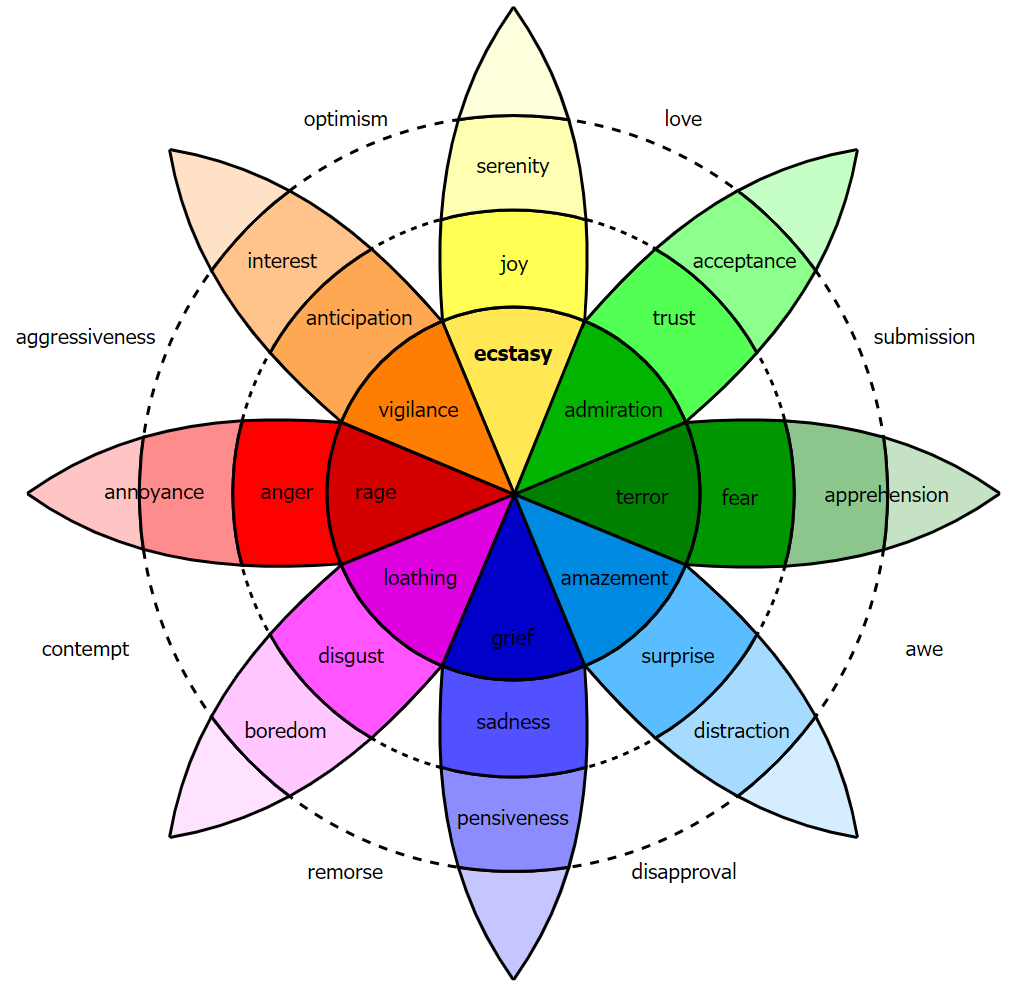
\includegraphics[width=0.72\linewidth]{plutchik_wheel.png}
	\caption{Plutchik Emotion Wheel}
	\label{fig:wheel}
\end{figure}

Similarly, the psychiatrist and philosopher Dr. Neel Burton speaks of the positive feelings of elation as states of euphoria, arriving at the pinnacle of ecstasy. He contends that ecstasy can be a route to epiphany, a sudden and striking realization, or as the Sanskrit root implies, ``a rising wisdom\cite{burton_heaven_2015}.''

This discussion reveals a problematic ambiguity. There is a strong association between ecstasy and happiness or joy, and this misdirects the vital impact of a truly ecstatic experience. The process of becoming ecstatic \emph{can be} joyful, yet drawing, for example, from the emotions in the final ring of the emotional wheel, it is easy to claim that the state of ecstatic mind, as reflected in innumerable accounts, can be equally frightful, grievous, astonishing, loathsome, or fascinating.

Wilhelm Mayer-Gross, a German-born (1889) psychiatrist, wrote his doctoral thesis on the subject of heightened emotion. In his analysis, The Phenomenology of Abnormal Emotions of Happiness, he reviews the literature of self-reported ecstatic experiences, often religious, contrasting with the documentation of psychiatric patients in the throes of mania\cite{mayer-gross_translation:_nodate}.  Mayer-Gross lays out what he considers six basic differences between ecstasy and abnormal happiness. Not to list them all here, the key feature repeated throughout is the observation that ecstasy can swell to displace the phenomena of an external world, to include one's own physical body, whereas happiness retains connection to external objects and phenomena, often as the subject or source of the state of joy itself \cite{beer_nature_2000} . Mayer-Gross refers to this total objective transformation as a dissolution of the self, and this is consistent with the overwhelming majority view from expert scientists, theologians, shaman, and ``ordinary'' people, who contend the overall effect of the ecstatic state is \emph{ego-dissolution}.

As it pertains to the remainder of this writing, the heightened emotional experience of ecstasy is understood as a transformation through exhilaration, of ego-dissolution, and a temporary reprise from the ordinary perceptions of the Self-in-World.

% --------------------------------------------------------------------------
% -- 
\clearpage


\chapter{Ecstatic Consciousness}
\noindent
{%
\setlength{\fboxsep}{0pt}%
\setlength{\fboxrule}{1.5pt}%
\fbox{
\includegraphics[width=\linewidth]{shaman_head.png}}%
}%
\label{Chapter:EcstaticConsciousness}

\emph{\ldots to be or stand outside oneself}\\

As the ecstatic experience relates to an altered state of perception of Self in a world of sensation, and establishing that a departure to said state can be triggered by combinations of experimental doses of nothing (i.e., no exogenous chemicals) and doses of something (e.g., 20 micrograms of DMT), it has been remarked by practitioners, shamans, spiritual leaders, gurus and researchers alike, that psychoactive drugs can be training wheels for the nascent enlightenment achieved through meditation. The directionality of the reference insinuates a preference for meditation, perhaps as a more respectable, if not at least legal, action. The machinations of materialistic cultures being what they are, society prides itself on sober problem solving and is therefore willing to tolerate meditators, while shunning self-medicated drug-users \cite{noauthor_war_nodate}.

\section{Altered States}


The idea of ``self-medicating'' is worthy of further discussion. Scientific advances in biology and organic chemistry triangulate to arrive at contemporary medical practices that condition modern people with the expectation that drugs are medicine for illness. Doctors are specialists who train in the fields of medicine, focusing in select domains or modalities. In a conventional, allopathic practice, they will analyze the complaints of patients, diagnose illness, and then select from a library of formulated solutions to manage the presumed illness, or, more frequently, only treat the symptom. Often the solutions are pharmaceutical---medicine for sick people. These proffered formulations are rarely foods or naturally occurring plants, but instead strictly regulated synthetic drugs. Many pharmaceutical synthetics emulate natural sources that may conceivably be growing in the parking lot or could be sourced from foods known to be high in the active ingredients. However, without a personal and casual relationship with healers, recommending a carefully managed diet, changes in destructive habits, or just common-sense behavior, exposes the system to unverifiable patient compliance, and professional liabilities. With the myriad dangers of our increasingly toxic environments, stressful schedules, and unhealthy habits, it is clear to see how a powerful and impersonal prescription drug culture might inevitably arise as the dominate medical ethos. This is not to say that modern medical science and synthetic pharmaceuticals do not have remarkable life-saving outcomes. Rather, the observation is of the tendency to believe exclusively in the techniques of technology as sacrosanct, approval by trusted authority, forgoing the subtler solutions presented in the natural world, which may be ancient, forgotten, or just too weird.

The converging of these factors has a chilling effect on the public`s will to explore consciousness transformation through psychoactive ritual. Most countries on Earth have made entire classes of psychoactive drugs illegal. The subject matter is effectively taboo. Returning to the academic investigation of consciousness and ecstasy, one must be cautious of falling for the societal tendency of rating the ethics between meditation and [illegal] drug-use. After all, consciousness itself appears to be agnostic to technique, and therefore any judgment regarding practice should remain subjective to individual values (and the aforementioned laws).

Let us observe that deviation from ordinary frames of reference, as shown by the recordings of ecstatic voyagers, may guide participants to beneficial states of mind. Evidence has shown altered mind states can have lasting therapeutic effects for mood disorders, assist in overcoming chemical addictions, and enhance overall peace of mind. With the postulate that the interplay of observing one`s \emph{self} in the world \emph{unexpectedly reframed} leads to ecstatic experiences, what are the specific ways to access ``reframing''---to alter conscious state?

\subsection{affective disorder}

Altering the state of mind is not exclusively a radical, nor is it exclusively an intentional process. Taken literally, altering state occurs at every instance of time as the conscious mind compares a persistent frame of reference from the cumulative past to perceptions of the present moment. Altering state is merely updating the present frame of reference. It is the intensity of alteration that qualifies for distinction as ecstatic. There are examples of ecstatic experiences that occur without the intentional or willing participation of the subject. Such an occurrence might be termed revelation when associated with beneficial foresight, or spiritual fervor. Often in the material and scientific world, spontaneous revelation is dismissed as psychosis.

A 1937 paper by EW Anderson, a clinician at the Cassel psychiatric Hospital in London, documents the study of four patients with a variety of affective disorders who experience bouts of ecstasy \cite{anderson_clinical_1938}. Anderson references E Blueler's Textbook of Psychiatry to define ecstasy as a ``\ldots states of rapture'' in which the outer world is completely interrupted. \enquote{The patients see the heavens open, associate with the saints, hear heavenly music, experience wonderful odours and tastes and indescribable delight of distinct sexual colouring that pervades the entire body.} 

The patients reviewed in the paper were admitted voluntarily and suffered from mild mood or personality afflictions that made them more of a nuisance than a threat to their communities. They moved through various states of psychiatric care before being referred to the hospital. While in the care of the facility, each had one or more ecstatic interludes featuring states of extraordinary calmness, bliss, and disassociation from the normal world. One patient described:

\begin{quote}
{There seemed a trembling vibration over my consciousness, a veil between me and what I should know, as if I were hovering beyond a great mystery. Then a dawning sense of exquisite harmony, without being lifted into the first state of ecstasy\ldots Thought, space, and time dropped away.}
\end{quote}
  
Anderson compared the descriptions to phenomena the late \nth{19} century psychiatrist RM Bucke called ``cosmic consciousness.'' He concludes that patients' inner tranquility and harmony with the environment was characteristically distinguishable from states of hyper mania. These were not psychotic manic episodes, but inexplicable phases of ecstatic delight.
A more recent paper (1987) about a much older case, neuroscientist D Landsboroug examines biblical references to ecstatic visions ascribed to the apostle Paul. In his letters to the Corinthians, Paul describes ecstatic experiences paired with ``a thorn in his flesh'' that are characterized by depersonalization, a connection to heaven, and auditory revelation [Figure \ref{fig:paul}]. Paul writes:

\begin{quote}
{I simply know that in the body or out of the body this man was caught up to paradise and heard sacred secrets which no human lips can repeat. Of an experience like that, I am prepared to boast\ldots My wealth of visions might have puffed me up, so I was given a thorn in the flesh, an angel of Satan to rack me and keep me from being puffed up.}\cite{bible_new_1984}
\end{quote}

\begin{figure}[h!]
	\centering
	{%
		\setlength{\fboxsep}{0pt}%
		\setlength{\fboxrule}{1.5pt}%
		\fbox{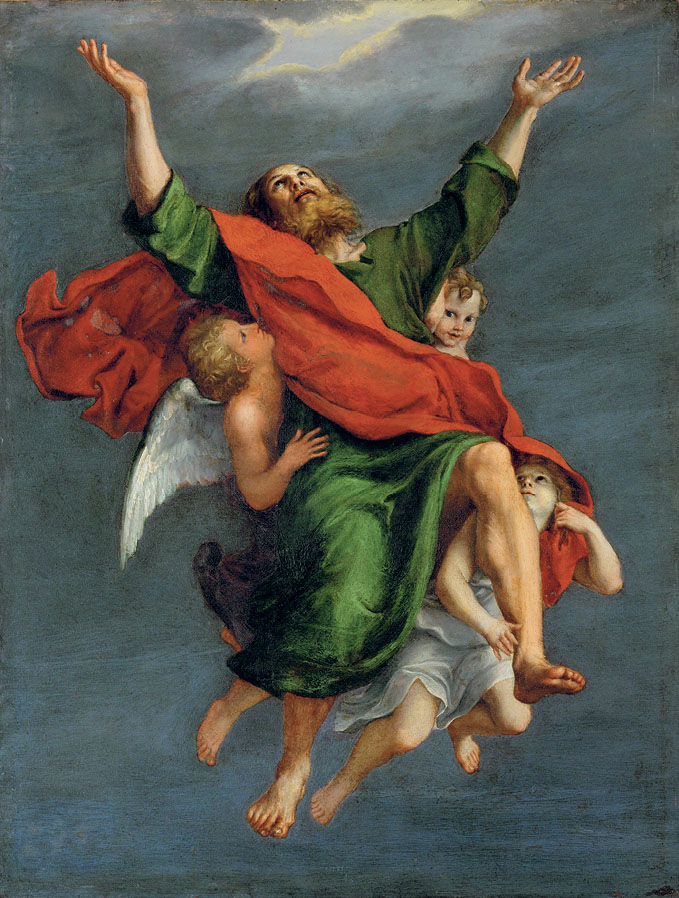
\includegraphics[width=0.63\linewidth]{paul.jpg}}%
	}%	
	\caption{Domenichino---The Ecstasy of St Paul, \nth{17} c.}
	\label{fig:paul}
\end{figure}

Paul's ``puffed'' up could mean too prideful, or boastful, from receiving such holy ecstasy. Realizing that he could lose touch with humble piety, he accepts his ``thorn'' as a mortal limitation, a sin physically manifest, retaining his station in the divine order. Landsboroug postulates that both the visions and the thorn were manifestations of temporal lobe epilepsy---a brain disorder that causes seizures and periods of unusual behavior or feelings.

As can be imagined, the debate over the nature of St Paul's thorn has raged for nearly two thousand years. A more recent author, Fyodor Dostoevsky, also had epilepsy. Written in 1868, \emph{The Idiot} tells the story of a young Russian noble returning to St Petersburg following a four-year commitment to a Swiss sanitarium for treatment of his epilepsy. Dostoevsky infuses his character with momentary ecstasy at the brink of each seizure:

\begin{quote}
{\ldots His sensation of being alive and his awareness increased tenfold at those moments, which flashed by like lightning. His mind and heart were flooded by a dazzling light. All his agitation, doubts, and worries seemed composed in a twinkling, culminating in a great calm, full of understanding\ldots}\cite{bible_new_1984}
\end{quote}

Other abnormal cognitive afflictions are known to trigger ecstatic episodes. In the article, The Nature, Causes, and Types of Ecstasy, MD Beer unearths several early \nth{20} century psychiatry trials reflecting on schizophrenic ecstasy and the resulting elation of manic episodes of disassociation, other-worldly visitations, voices, and hallucinations \cite{beer_nature_2000}.

While the involuntary occurrences of affective disorders may occasion an ecstatic response in persons so afflicted, it is also well understood that a voluntary engagement with ecstasy may be actively courted with the practiced discipline of meditation.

\subsection{meditation}
Considering the features of meditation provides further insight into the mechanisms of conscious expanding ecstasy. For the sake of simplicity, meditation discussed here represents the collection of methods focused on changing state of mind though voluntary, sustained, disciplined techniques, to include controlled breathing, chanting, prayer, drumming, dancing, fasting, mindfulness, and silent retreat. Unlike affective disorders or psychoactive drugs, both of which overpower processing behavior in the central nervous system, the key to meditative ecstasy is non-invasive, sustained, and intentional techniques.

Meditation may source a secular credo, but due to the influence of organized religion, and the literary nature of religious scholarship, documentation of meditation/prayer that is of religious or spiritual nature is widely available. The monotheistic lineages of the middle east focus almost exclusively on the historical preservation of divine revelation as received by prophets and apostles. Those references are minimally useful; perhaps best as anthropological clues as to the evolving historical importance of ecstatic ritual at the cultural level.
 
While it is true that monotheists developed a monastic class that spend time in isolated prayer and study, and this undoubtedly qualifies for meditation, the Eastern spiritualities document a wide variety of technique for approaching ecstasy from an individual perspective. Yogic traditions drawing upon the ecstatic forms of meditation are thousands of years old. The Yoga-S\^{u}tra, Bhagavad Gita, Pata\~{n}jali, Vij\~{n}\^{a}nabhairava, and Pratyabhij\~{n}\^{a}hrdayam are classical yoga texts describing ecstatic meditation \cite{waelde_dissociation_2004}.

For example, tradition based on the Vij\~{n}\^{a}nabhairava, a compendium of 112 yoga techniques delivered in verse, guides practitioners to control the mind through disciplined observation. Yogis learn to control state of mind by directing attention away from the senses by, for example, watching the breath, repeating mantras, or evoking visualizations. Verse 104 says to achieve happiness, the yogi should reject identification with his body in favor of the inner Self. 

Lest it appear that The Vij\~{n}\^{a}nabhairava requires a practitioner to deny one part of reality, in preference for another (which the act of perceiving, by process, also must do at every moment) consider a practical example of another verse, which asks the disciple to meditate on the joy of seeing a long-missed friend, so that the mind becomes absorbed in the feeling of joy \cite{singh_vijnanabhairava_2002}.

It is not necessary to rely on the stories of ancient texts and spiritual anecdotes alone. A multi-institutional case study published in 2013 demonstrated that highly trained meditation practitioners are capable of generating and sustaining self-stimulating brain states. Researchers studied a Buddhist concentration technique called jhana that induces \textit{\ac{ASC}} in a series of eight sequences [Figure \ref{fig:graphjoy}]. The study methods included \textit{\ac{fMRI}} and \textit{\ac{EEG}} recordings to observe a Buddhist with 17 years of meditation practice. 

The research concluded five distinct features of the subject's conscious state, (1) external awareness dims, (2) internal verbalizations fade, (3) the sense of personal boundaries is altered, (4) attention is highly focused on the object of meditation, and (5) joy increases to high levels \cite{michael_r._hagerty_case_2013}.

\begin{figure}[h!]
	\centering
	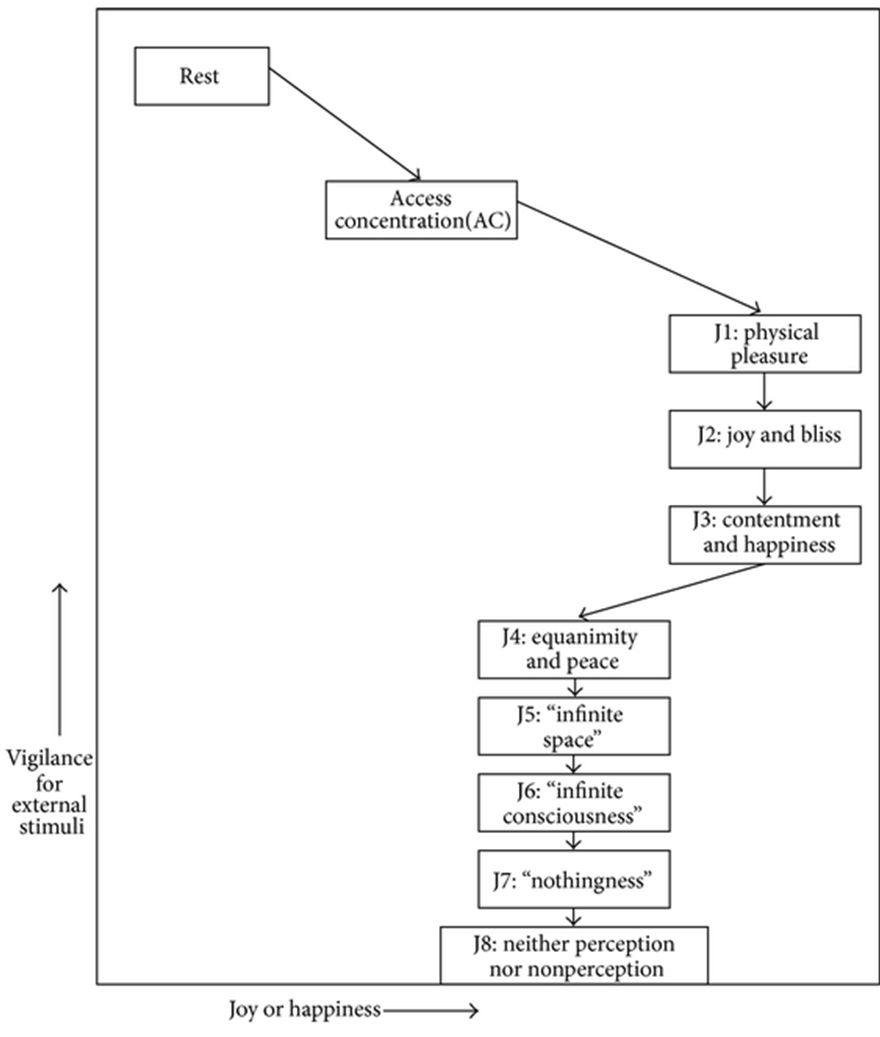
\includegraphics[width=0.63\linewidth]{graph_joy.png}
	\caption{Schematic of the reported experiences in 8 jhanas relative to resting consciousness and concentration on 2 dimensions of interest; \emph{joy or happiness}, and \emph{vigilance for external stimuli}.}
	\label{fig:graphjoy}
\end{figure}



Disciplines like these achieve a practical application, by freeing the individual from undesired effects of worldly phenomenon. Can we consider a skilled meditation practitioner the beneficiary of a sustained ecstatic mind?

Accepting that the disciplined intent of meditation can expand consciousness, let us consider the impact of psychoactive chemicals which portend to achieve analogous effects. 


\subsection{entheogens}

An entheogen is a psychoactive substance used in a spiritual or shamanic context. The term was first coined in 1979 by Ruck, Bigwood, Staples, Ott, and Wasson \cite{ruck_entheogens._1979}, meaning ``becoming the god within'' or ``becoming divine within.''  Entheogens may be directly gathered from natural plant sources, as in mushrooms or cactus flowers; may be brewed from combinations of plants, as in ayahuasca; or may be wholly synthetically derived, like LSD, MDMA, and DMT. Entheogens contain molecules closely related to endogenous neurotransmitters. 

When he was sixty years old, the coincidental Father of LSD addressed the 1966 Worlds of Consciousness Conference in Heidelberg: \enquote{Mystical experiences in [my] childhood, in which Nature was altered in magical ways, had provoked questions concerning the essence of the external, material world, and chemistry was the scientific field which might afford insights into this.} Forty-two years later, Albert Hofmann died at his home in Switzerland, 102 years old.

Dr. Hofmann joined the pharmaceutical-chemical department of Sandoz Laboratories in Basel as a lab chemist. He was working on synthetic derivatives of fungus ergot in 1938 when he developed a series of analogs that failed to produce the intended goals in the laboratory test animals. The formulations were abandoned for five years, until he self-initiated an informal study of one variant, LSD-25, to satisfy a lurking curiosity.
In the handling of the chemicals in the lab on the day of the reboot, Hoffman incidentally absorbed compound from the crystallized tartrate salt product. He sent the following report to the head of the lab, Arthur Stoll:

\begin{quote}
{Last Friday, April 16, 1943, I was forced to interrupt my work in the laboratory in the middle of the afternoon and proceed home, being affected by a remarkable restlessness, combined with a slight dizziness. At home, I lay down and sank into a not unpleasant intoxicated-like condition, characterized by an extremely stimulated imagination. In a dreamlike state, with eyes closed (I found the daylight to be unpleasantly glaring), I perceived an uninterrupted stream of fantastic pictures, extraordinary shapes with intense, kaleidoscopic play of colors. After some two hours, this condition faded away.}\cite{hofmann_lsd:_1980}
\end{quote}

Hoffman had unintentionally become the first person on Earth to have an acid trip. His report to Professor Stoll a few days later demonstrates the well-documented occurrence of \emph{closed-eye hallucinations}. In psychedelic drug culture, hallucinations are frequently a goal of recreational drug users. Fanciful, colorful, elaborate, the styles of visual hallucinations are the hallmark signature of psychedelic art and memorabilia. 

This feature of visual sensation without any light entering the optic system opens inquiry into the nature of consciousness and perception. Famed neurologist Oliver Sacks published his penultimate book, \emph{Hallucinations}, detailing case studies of sensory distortions triggered by fever, injury, drugs, sensory deprivation, exhaustion, and grief. One patient was completely blind, but never-the-less `saw' innumerable visions, including extraordinary specific details of children in brightly colored Eastern clothing, and elves and faeries climbing the sides of her wheelchair. Sacks explains the brain needs not only perceptual input but perceptual change, and that the ``deprivation of normal visual input can stimulate the inner eye'' to produce dreams or hallucinations \cite{sacks_hallucinations_2012}.

Considering these stories of hallucination, whether triggered by bruising the brain falling down a staircase or ingesting \SI{250}{\micro\gram} of LSD, one is hard-pressed to locate within a functional role for a consciousness-expanding ecstatic journey. What use is a fleeting perceptual ``aberration''?

Turning back to the story of Albert Hoffman, three days following his unintended preeminent exposure, he returned to his lab to subject himself to a controlled experiment. Informing a lab assistant of his intentions, he cooked up another batch and measured out what he thought was a safe threshold dose of LSD. Today we know that threshold dosages are in the 10-\SI{20}{\micro\gram} range, with a ``strong'' dose falling between 150-\SI{400}{\micro\gram}. Hoffman took \SI{250}{\micro\gram}.

Within 40 minutes, feelings of anxiety, dizziness, and visual distortions began. He felt in crisis, finding it difficult to speak, but was able to communicate with the assistant that he needed an escort home. On April 17, 1943, Albert Hoffman, under the influence of powerful LSD hallucinations, rode his bicycle home. In his book published in 1979, LSD, My Problem Child he describes the terrifying feelings he endured during the peak of his intoxication, an estimated two hours. Of the following day he writes, 


\begin{quote}
{Exhausted, I then slept, to awake next morning refreshed, with a clear head, though still somewhat tired physically. A sensation of well-being and renewed life flowed through me. Breakfast tasted delicious and gave me extraordinary pleasure. When I later walked out into the garden, in which the sun shone now after a spring rain, everything glistened and sparkled in a fresh light. The world was as if newly created. All my senses vibrated in a condition of highest sensitivity, which persisted for the entire day.}\cite{hofmann_lsd:_1980}
\end{quote}


\begin{figure}%[h!]
  \centering
  \begin{subfigure}[b]{0.4\linewidth}
    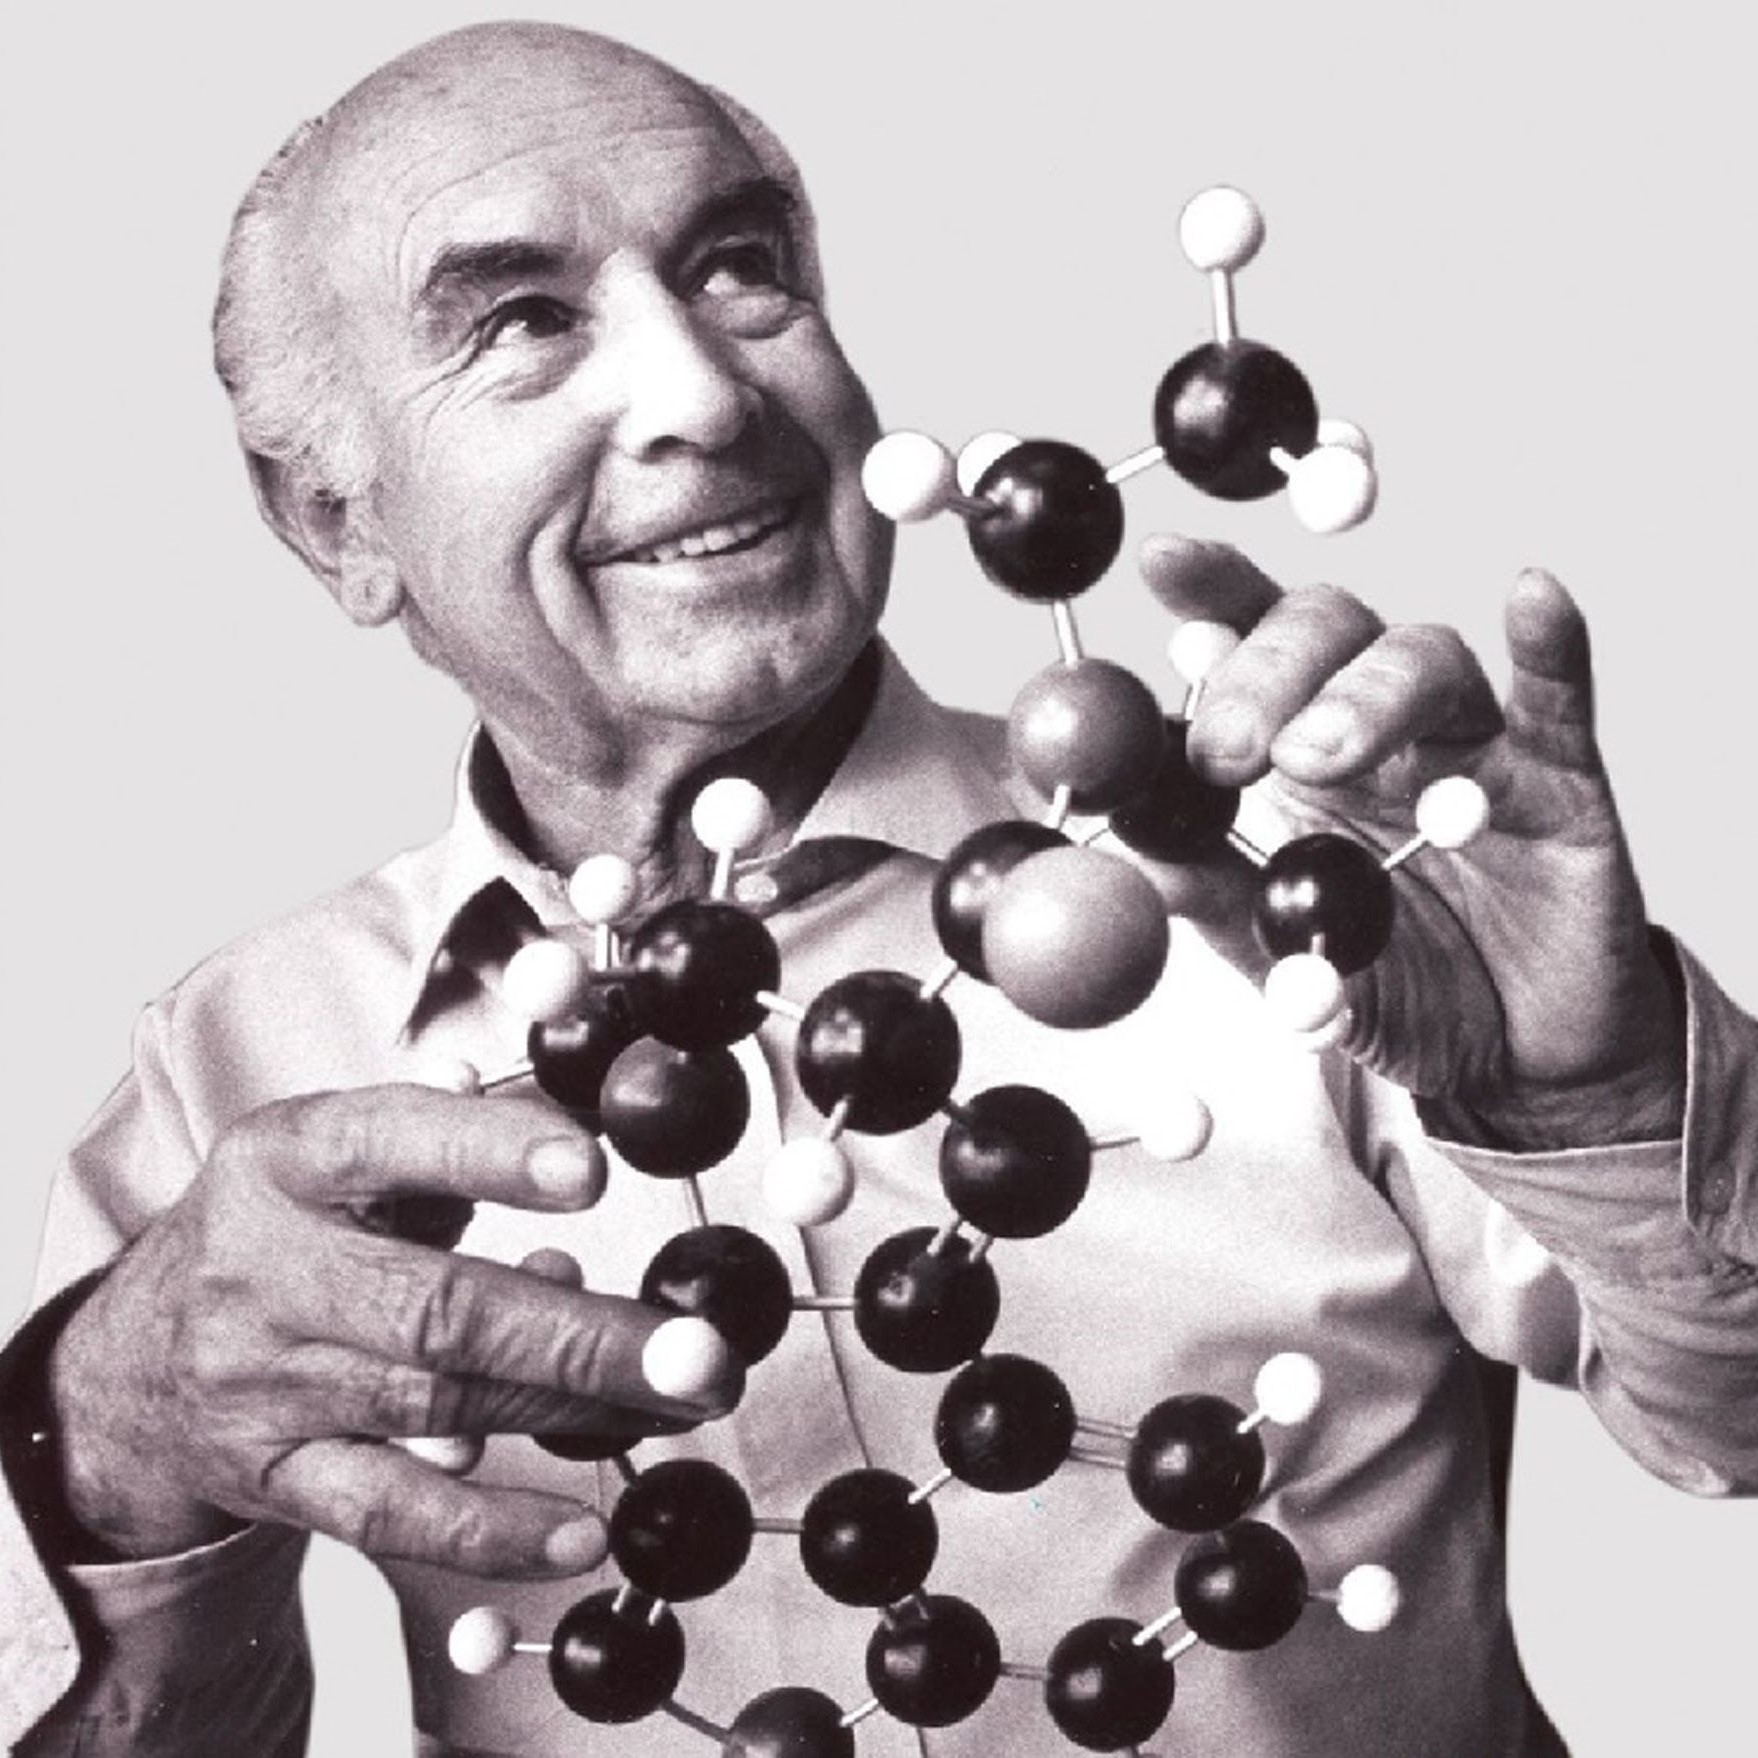
\includegraphics[width=\linewidth]{hofmann_sq.jpg}
    \caption{Dr. Albert Hofmann.}
  \end{subfigure}
  \begin{subfigure}[b]{0.4\linewidth}
    
\includegraphics[width=\linewidth]{bicycle_day.jpg}
    \caption{Bicycle Day - blotter acid}
  \end{subfigure}
  \caption{LSD: Hofmann's \enquote{Problem Child}}
  \label{fig:hofmann}
\end{figure}

The dissidence of comparing fun-loving hallucinating psychedelic trips to the ecstatic experience of ritualistic entheogen trance is reflected on by Ralph Metzner, a pioneer in psychological and cross-cultural studies of consciousness expansion. He is a psychotherapist and professor emeritus at the California Institute of Integral Studies. In his 2017 publication, \emph{Entheogens: Toward an Expanded Worldview for Our Time} he writes,

\begin{quote}
{Whereas the terminology of psychedelics has acquired spurious cultural associations of `tripping,' the historically primal concept of consciousness expansion has two advantages. One, it connects psychedelic drugs with other modes of consciousness expansion, such as meditation and creative visioning; and two, it suggests contrasting comparison with the consciousness contraction involved in concentration and focus.}\cite{metzner_entheogenesis:_2017}
\end{quote}

Whether drug use helps an acolyte to learn the routes to achieve ecstatic meditation, or meditation encourages or works in tandem with entheogenic drug ritual, it is not the focus of this work to take up the position on the primacy of one of these positions over another. Such debate is best left to philosophers, and while we must bear it, legal states who deem it their right to mediate.

\section{A Pscychoactive History}

From the contemporary perspective of Western Civilization, there is little to no expectation for individuals to engage states of ecstasy for beneficial personal growth. Case in point, the drug MDMA invented by German chemists in 1912, would become popularized in the 80s as Ecstasy. Subsequently, the vernacular occurrence of the word has been dominated by the reference to the drug, not the feeling or emotional state for which it was named. To casually verify this assumption, a Google Ngram publication report from 1900-2008 shows the rise in incidence for the term ecstasy to refer to the popular club drug over the emotional state, to eventually rank five times more frequent by the end of the \nth{20} century. [Figure \ref{fig:ngram}]

\begin{figure}[h!]
	\centering
	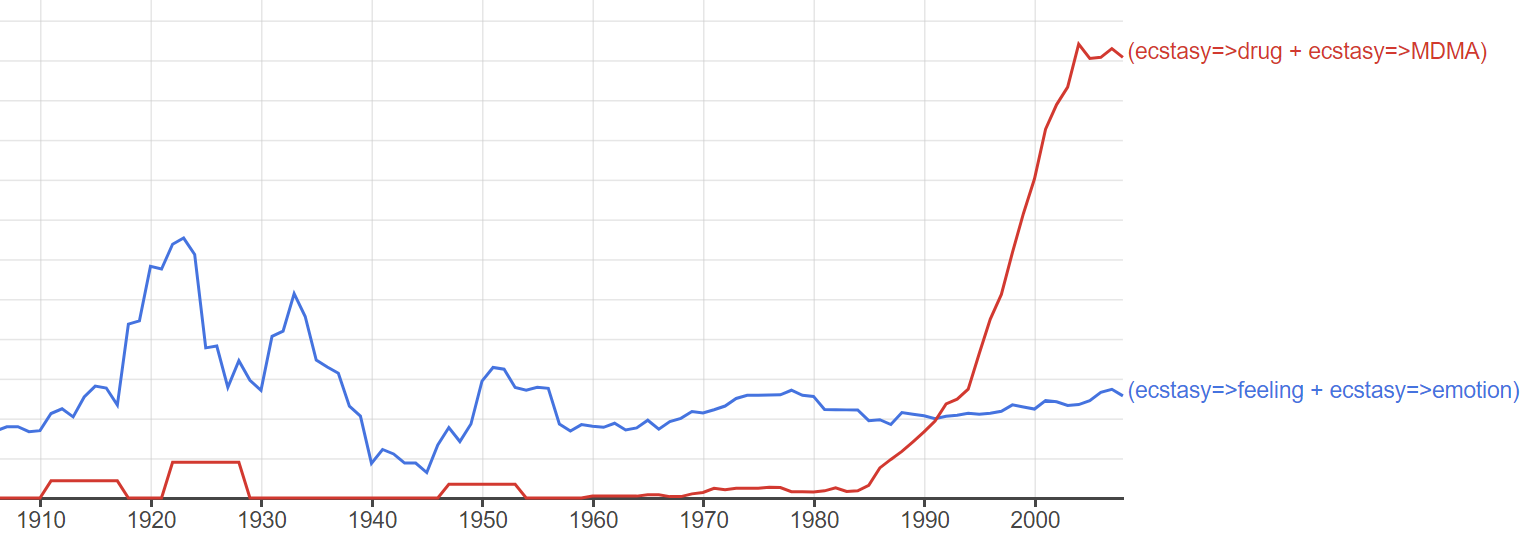
\includegraphics[width=\linewidth]{ecstasy_ngram.png}
	\caption{Google Ngram - ecstasy vs Ecstasy}
	\label{fig:ngram}
\end{figure}

One takes little comfort from the realization that the use of the word `ecstasy' has been trumped by a drug called Ecstasy that assists the user into a \emph{state of ecstasy}. This word ambiguation has an effect of diminishing the concept of emotional ecstasy in popular English language. When the reader hears the word `ecstasy' with minimal context on any given occasion, which occurrence comes to mind? Symbolic language is an imperfect tool.
 
This discussion can be confusing as it relies on subtle cultural inferences to make the point that many of the first wave anthropologists, scientists, and spiritual seekers who rediscovered existing drug ecstasy cultures or created the opportunity for entirely new ones in the laboratory, oft times reported regret for bringing casual public light to the heretofore unknown or forgotten substances. The frivolous, untrained, unserious use of mind-altering drugs, as expressed in pop culture, does encounter some risk. 


\subsection{psychedelic genesis}

The fascinating story of Gordon R Wasson tells of one such de facto anthropologist. A New York city banker by profession, Wasson was a pharmacological nonentity with no experience in chemistry or formal anthropology. In 1955 he and a photographer named Allan Richardson mounted a mission to the Mixeteco mountains of central Mexico to track down rumors of mystical mushrooms revealed in an obscure ten-year-old botanical journal.

There they met the Mixtec people and became the first white people in known history to participate in ceremonial consumption of \emph{divine} Psilocybe mushrooms. Wasson and his wife Valentina P Wasson, MD, would return each summer to the region, inquiring into the varieties of magic mushroom, and the rituals of their stewards.

In 1957, Life magazine published a multi-page article written by Gordon Wasson, detailing aspects of his experience. The article included several full-page photos and carefully drawn artwork depicting a variety of mushroom species. The article sparked tremendous interest in the funny `shrooms', inspiring a psychedelic tourism of hippies and beatniks seeking trippy times. The psychedelic revolution had begun. 

Sadly, the onslaught of questing visitors brought the attention of the Mexican police, threatening the Mixtec rituals and way of life. The medicine woman who originally shared her secrets with the Wassons was eventually ostracized from the community, and her house was raised, presumably by her people.

In roughly the same timeframe, the psychologist Humphrey Osmond had established a hallucinogenic drug study at the Weyburn Mental Hospital in Saskatchewan. Osmond had worked for a few years with mescaline and then transitioned to treating alcoholics with LSD. Of 2000 patients treated, Osmond reported that 40-45\% did not return to drinking after one year \cite{dyck_hitting_2006}.

Aldous Huxley, the British writer, known for the epically dystopian novel \emph{Brave New World}, had learned of mescaline and Dr. Osmond. He established a correspondence with Osmond, then, in 1953, Osmond introduced Huxley to the substance. \emph{The Doors of Perception} was published the following year; a 63-page philosophical essay detailing his trip.

In their subsequent friendship and correspondence, we witness the birth of the term psychedelic. Osmond instigated a dialog with the writer in search of a name for the effect of LSD on the mind. Huxley suggested \emph{phanerothyme}, from the Greek for ``to show'' and ``spirit,'' then promoted the term with a rhyme \enquote{To make this mundane world sublime, Take half a gram of phanerothyme.} Osmond countered with \emph{psychedelic}, from the Greek \emph{psyche} ``mind'' or ``soul'' and \emph{deloun}, ``show'', demonstrated in the shibboleth \enquote{To fathom Hell or soar angelic, Just take a pinch of psychedelic.} Osmond announced the new term at the 1957 New York Academy of Sciences meeting. 

\newpage

\begin{figure}[h!]
  \centering
  \begin{subfigure}[b]{0.4\linewidth}
    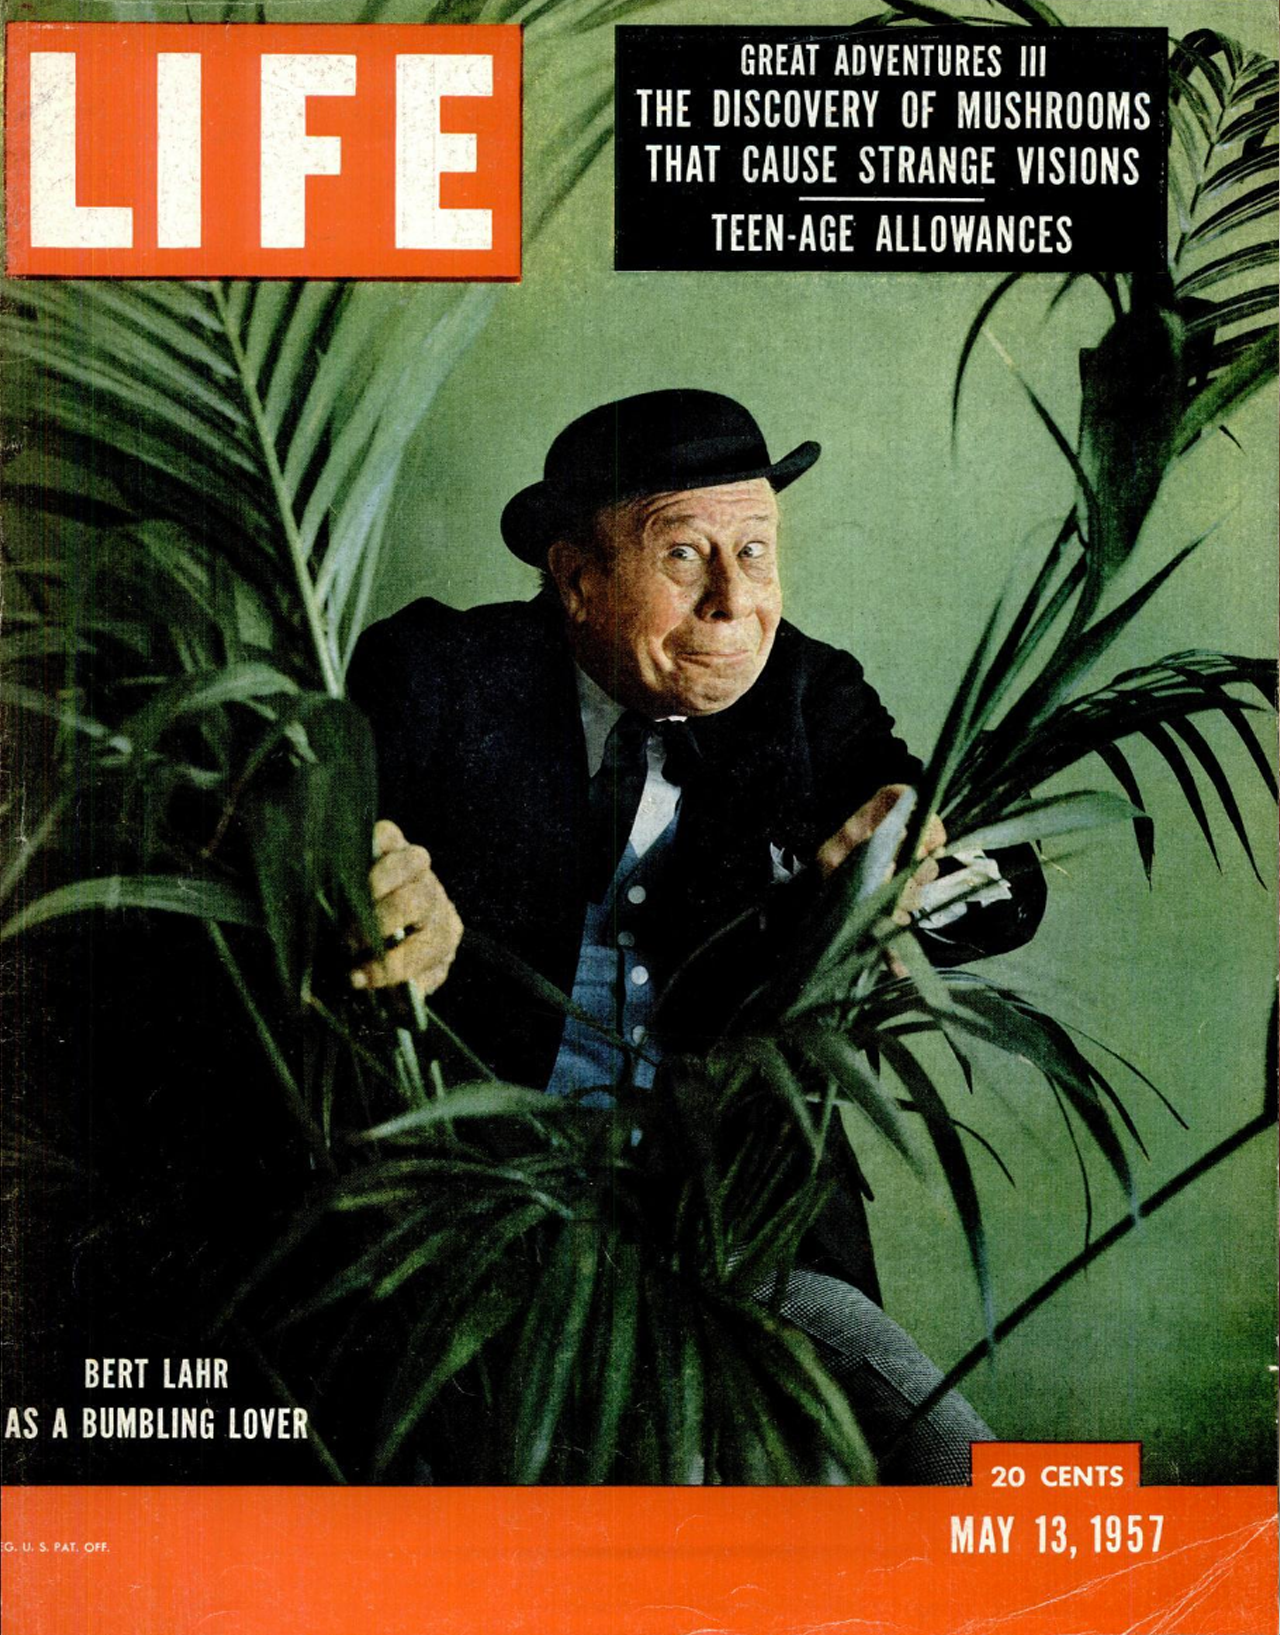
\includegraphics[width=\linewidth]{life57.png}
    \caption{Life 1957 - Seeking the Magic Mushroom}
  \end{subfigure}
  \begin{subfigure}[b]{0.4\linewidth}
    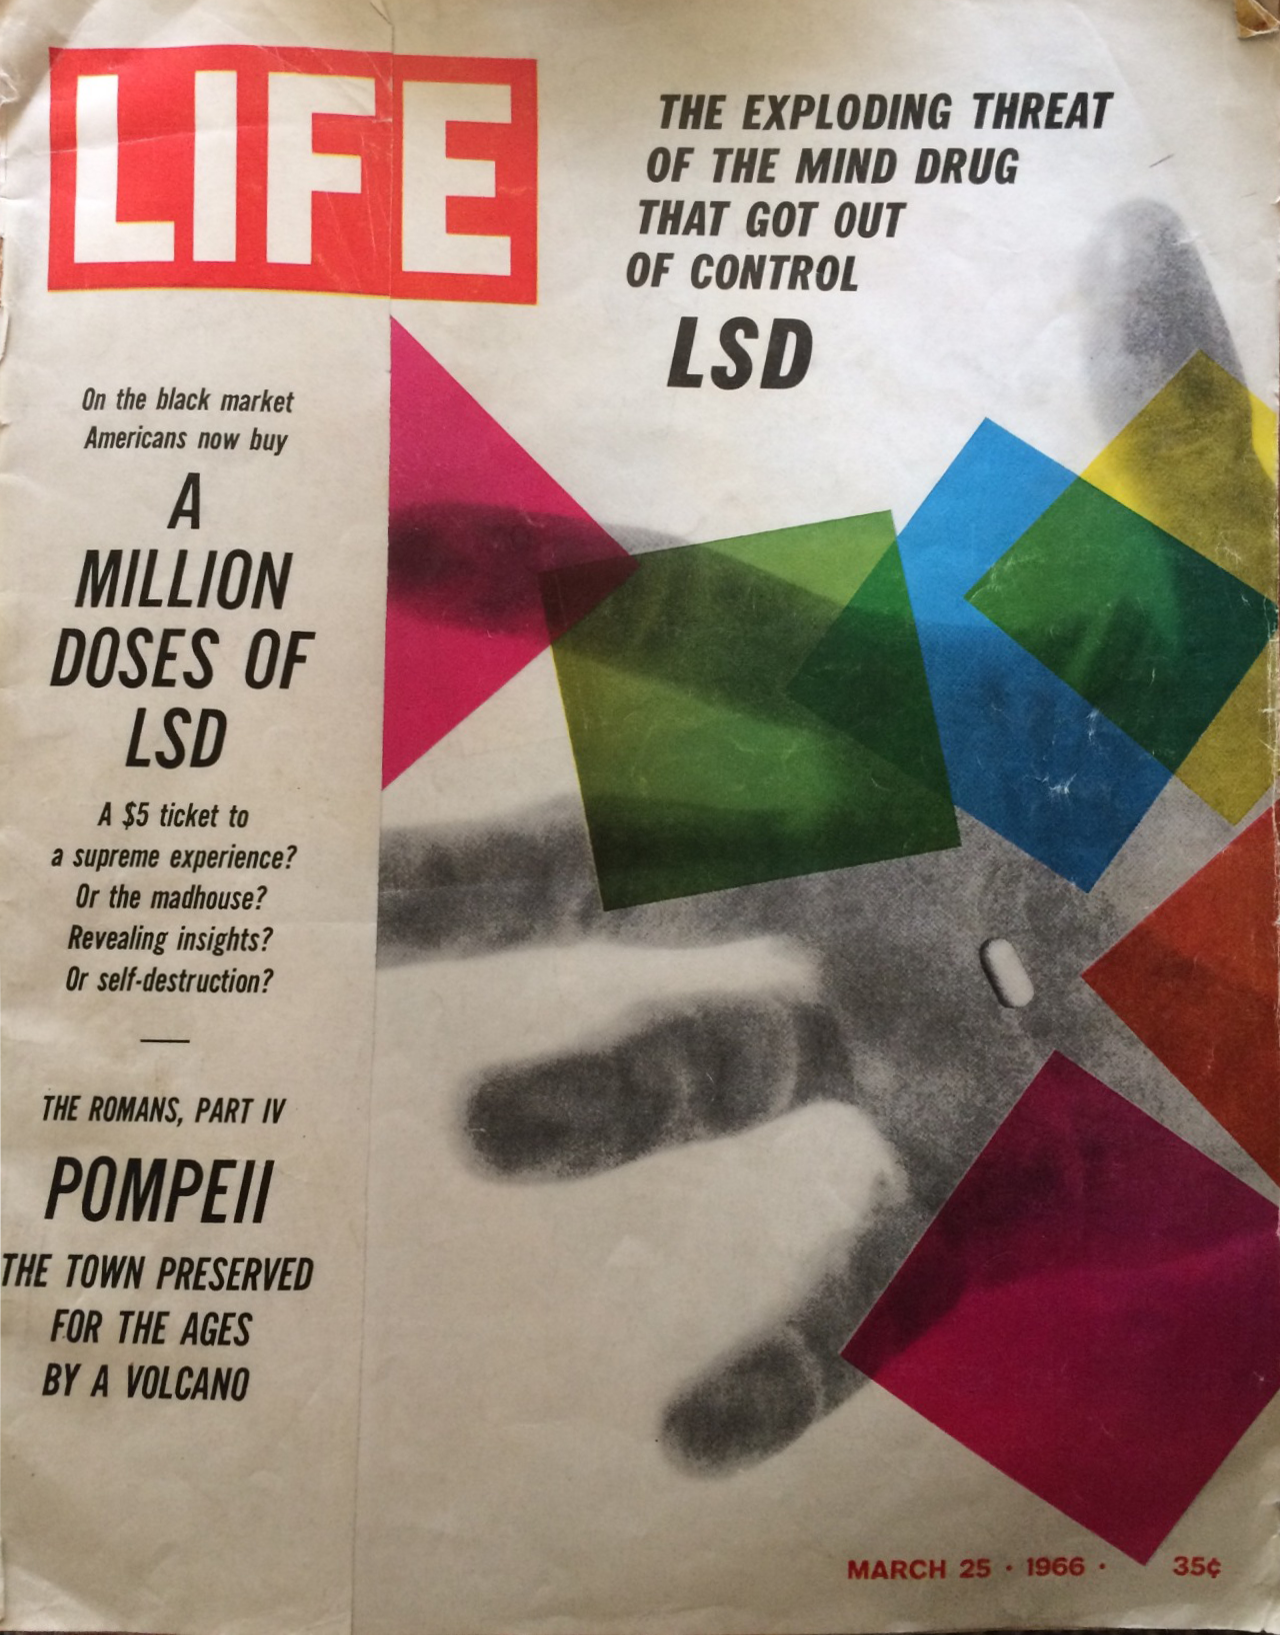
\includegraphics[width=\linewidth]{life66.png}
    \caption{Life 1966 - A Remarkable Mind Drug Suddenly Spells Danger}
  \end{subfigure}
  \caption{American's change of heart for psychedelics}
  \label{fig:hofmann}
\end{figure}

\subsection{psychedelic revolution}
\epigraph {Psychedelic drugs cause panic and temporary insanity---\\
in people who have not taken them!}{Timothy Leary 1963}

\vspace{9mm}

Wasson's article soon attracted the attention of a notable Harvard psychologist, Dr. Timothy Leary. A colleague, Anthony Russo, confirmed the veracity of the claims, having also made the journey to Mexico. In August of 1960, Russo accompanied Leary to Cuernavaca, Mexico, where he consumed psilocybin mushrooms for the first time. Of that first encounter, Leary is know to have said that he \enquote{learned more about\ldots (his) brain and its possibilities\ldots more about psychology in the five hours after taking these mushrooms than\ldots in the preceding 15 years of studying and doing research in psychology \cite{dassfierce}.} 

Within the year of his preeminent ecstatic psilocybin experience, Leary and his colleague Richard Alpert, together with board member Aldous Huxley, formed the Harvard Psilocybin Project, to document the effects of psilocybin on human consciousness. Recall that in that time, neither LSD nor psilocybin was classified substances. The team ordered psilocybin from the Sandoz lab, where Albert Hofmann had developed the process to derive the compound synthetically \cite{melechi_psychedelia_1997}.

With a steady supply of psychoactive potion on tap, Leary and Alpert administered the drug to volunteers from the Harvard student body, other researchers, prison inmates, and a group of divinity students. Of the last group, the famed ``Good Friday'' experiment, the Project researchers dosed the experimental group with psilocybin while attending a Good Friday service in a private chapel. The effect from the combined influence of intense religious ceremony and iconography, with psychoactive neurochemicals yielded a dramatic emotional response in the experimental group. Leary claimed that with entheogens \enquote{spiritual ecstasy, religious revelation, and union with God were now directly accessible \cite{mansnerus_timothy_1996}.}

Controversy followed the program in short order. The team's experiments suffered from unconventional design, such as non-random subject selection, and lacked proper control groups. More damning was the practice of the researchers taking the drugs themselves along with the subjects. Intradepartmental opponents of the project charged that the studies ``resembled cocktail parties,'' and that their data collection was sloppy.

The project ended in under three years. Harvard denied Leary a new contract after he failed teaching obligations, preferring to travel during that semester. Alpert was fired for giving drugs to undergrads, which was against the standing agreement with the school. Ultimately both were banned from academia. In short order, Alpert went to India to study at the Kainchi ashram, where he accepted a new name, Ram Dass, ``servant of God.'' Subsequently, he made a lifetime commitment to the spiritual path of non-exogenous self-induced ecstasy via disciplined meditation and yogic practice. He published a seminal yogi guidebook, Be Here Now, in 1971, often described as a countercultural bible. He continues to publish books and produce media content and events with the Be Here Now Network.

Leary followed a very different path, directing his attention to a pro-active mass counterculture of psychedelic non-conformity. In a prelude to the 1967 Summer of Love, 30,000 hippies gathered in Golden Gate Park, San Francisco, for the Human Be-In event. In a speech to the crowd, Leary delivered his now-famous phrase, ``Turn on, tune in, drop out.'' Leary claims that Marshall McLuhan crafted the phrase and had given it to him during a lunch meeting. McLuhan spoke about the marketing power of jingles and slogans and began singing a ditty to the melody of a popular Pepsi commercial that went something like,\enquote{Psychedelics hit the spot; Five hundred micrograms, that's a lot. Tune in, turn on, and drop out.}

Leary also popularized the phrase ``think for yourself and question authority,'' which he must surely have donned as a mantel, for over the two decades following his Harvard dismissal, he had been in dozens of jails on multiple continents, an escaped fugitive, and finally extradited from Afghanistan. Richard Nixon dubbed him ``the most dangerous man in America.'' Ironically, it was not yet illegal to possess his infamous drug of choice, LSD, but the marijuana tax act of 1937 had teeth. Of two minor marijuana arrests, one he successfully defended in the Supreme Court in 1969 for a clever technicality; the second landed him at Folsom Prison, where he served 5 of a 30-year sentence \cite{higgs_i_2006}.

By the mid-1960s, the tide had turned against the psychedelic tricksters. The nation was involved in a continuing unpopular armed conflict in Asia, and a de facto cultural war at home fueled by a youthful dissent. Nine years following Life's mischievous light-hearted 1957 magic mushroom article, a new ominous cover story read \enquote{The Exploding Threat of the Mind Drug That Got Out Of Control: LSD} with an overleaf addition that claimed \enquote{A Million Doses of LSD: \$5 ticket to a supreme experience? Or the madhouse? Revealing insights? Or self-destruction?} This was a verbose sign (1966 readers had perhaps less panache for zippy cover copy than today) that the establishment had become unsympathetic to the psychedelic credo. In 1970, LSD, psilocybin, mescaline, peyote, DMT, and chemicals resembling DMT, were added to the US Controlled Substance Act under Schedule I, followed in 1971 by the United Nations Convention on Psychotropic Substances. 



\subsection{shamans}

The chilling effect of international embargo was hardly a new chapter. As we recall, it was only the cautious and nearly accidental discoveries of the early \nth{20} century, from laboratory chemistry, to hobbyist anthropologists, they brought both synthetic and naturally-occurring consciousness-expanding substances into public awareness. 

\section{Ecstatic Novelty}

The quest to explore ecstatic consciousness finds growing market support in the 21st century. An NIH survey of US adults over 18 reveals that 14.3\% of respondents practice yoga, and 14.2\% meditate.  Comparing data from 2012 to 2017, the 2017 figures are up five and ten points, respectively. The use of psychedelics is on the rise as well. LSD use increased 175\% among younger users in England and Wales between 2013 and 2015 \cite{gayle_ecstasy_2015}, and A 2004 population study in the US show over 30 million people living in the USA have used LSD, psilocybin, or mescaline. \cite{krebs_psychedelics_2013}

Jules Evans, a writer, philosopher, and research fellow for the Center for the History of Emotions, finds this intersection of interests bearing on the ideas represented by \textit{\ac{TP}}. A stoic philosopher, he never-the-less pens his second book publication, The Art of Losing Control: A Guide to Ecstatic Experience, Evans succinctly states, \enquote{I have decided that Western culture has a problematic relationship with ecstasy, and this narrows and impoverishes our experience of reality.}

A school of psychology integrating spiritual and transcendent human experience with a modern psychology framework, the field was established by turn of the century thinkers William James, Carl Jung, Abraham Maslow, and Roberto Assgili. The transpersonal is defined as experiences in which the sense of identity or self extends beyond (trans) the individual or personal to encompass wider aspects of humankind, life, psyche or cosmos \cite{calijornia1993transpersonal}

The ecstatic gateway to the transpersonal proposes an interesting relationship with the self. What begins as a uniquely subjective experience, exhilarates the perceiver beyond her personal boundaries, into an unfamiliar state beyond the self. The transpersonal is a liminal state between subjectivity and objectivity. Seeking ecstasy is a path beyond self, embracing the transpersonal.

\subsection{accepting the unknown}

Mass culture conditions individuals to be wary of deviation from the norm. While this is a clear tautology, it is nevertheless a useful note when questioning how public policy can prohibit an individual's right to eat something growing in the front yard. Terance McKenna has a few words to say about the flamboyant hubris of cultural authority

\begin{quote}
{Culture is not your friend. Culture is for other peoples' convenience and the convenience of various institutions, churches, companies, tax collection schemes, what have you. It is not your friend. It insults you. It disempowers you. It uses and abuses you. None of us are well-treated by culture. [\ldots] It fetishizes objects. It creates consumer mania. It preaches endless forms of false happiness, endless forms of false understanding in the form of squirrelly religions and silly cults. It invites people to diminish themselves and dehumanize themselves by behaving like machines.}
\end{quote}

McKenna's contentious notions aside, there are volumes of studies on the possible roles played by culturally transmitted conformity, in evolutionary biology as well as social psychology. If a member of your migrating band eats a strange plant along the trail, then keels over dead, perhaps negative reinforcement avoidance is a good starting point for your would-be cultural heritage.

It is well accepted that the astonishing advances of human knowledge owe many tributes to the sometimes dangerous exploration of the unknown. Simultaneously, there exists ample anecdote of cultural knowledge that is simply disregarded due to prejudice or ignorance. How much have non-western cultures, historical and concurrent, already known about the mind, the self, and the possible trans-selves? Modern man is prone to conceit and ethnocentrism, especially when addressing anything that appears to belong to the realm of material science.

William James (1842-1910), one of the architects of TP, made his mark at Harvard, helping to establish the psychology department in the late \nth{19} century. James is a colorful character in the history of psychology, studying first painting, before enrolling at Harvard to study chemistry and anatomy. The discipline of psychology was not discrete, but his interest in behavior lead him to study the mind and the nascent emergent field. \enquote{This is no science; it is only the hope of science,} he wrote in his 1892 survey, Psychology: Briefer Course. 

To the psychedelic researcher, his 1901 book, The Varieties of Religious Experience: A Study in Human Nature, provides much-cited prose for the abstract handling of human consciousness.

\begin{quote}
{Our normal waking consciousness\ldots is but one special type of consciousness, whilst all about it, parted from it by the filmiest of screens, there lie potential forms of consciousness entirely different\ldots No account of the universe in its totality can be final which leaves these other forms of consciousness quite disregarded \cite{james1961varieties}.}
\end{quote}

James' sentience about the possible fractal nature of mind was not the result of a lucid waking divinity. James had learned from the chemist and inventor Humphry Davy to use nitrous oxide to produce unexpected visions and insight into his consciousness. Based in part on his experiences huffing NO, James developed a four-point guide for defining mystical encounters \cite{popova_william_2018}.

\nohyphens{
	\subparagraph{Ineffability:} Inexplicable, defying expression and language. Requires direct experience.
	\subparagraph{Noetic quality:} True and deep insight; revelation; full of significance; durable
	\subparagraph{Transiency:} Fleeting in duration; difficult to recall in detail, but recognizable in subsequent revelation
	\subparagraph{Passivity:} The mystical state may be established voluntarily, but once it begins, the mystic is held beyond volition 
}

Neuroscience has come a long way since the James 1901 publication, but his mystical roadmap still makes handy short-shrift for wayfinding in even the most rigorous psychedelic research today.

Michael Pollan's recent book, How To Change Your Mind: What the New Science of Psychedelics Teaches Us About Consciousness, Dying, Addiction, Depression, and Transcendence, references James' contributions often. From the contemporary research scene, Pollan speaks to the head of psychedelic research at Imperial College, Robin Carhart-Harris, who likens the taking of psychedelics to ``shaking a snow-globe'' to free the brain from traveling in the ruts of aged conditioning.

Carhart-Harris explains that current models for understanding cognition support a feature of the brain called the default mode network. The \textit{\ac{DMN}} appears to be involved in this rut-like behavior---when anxious, insecure, or self-absorbed, the brain shows less potential activity, traveling well-established and potentially fruitless connections. A study using psilocybin on subjects with \textit{\ac{fMRI}} imaging published in 2014 concluded, \enquote{the effect of psilocybin is to relax the constraints on brain function, ascribing cognition a more flexible quality.} The imaging discovered [see figure \ref{fig:dmn}] that the DMN shuts down almost entirely. 

\begin{figure}[h!]
	\centering
	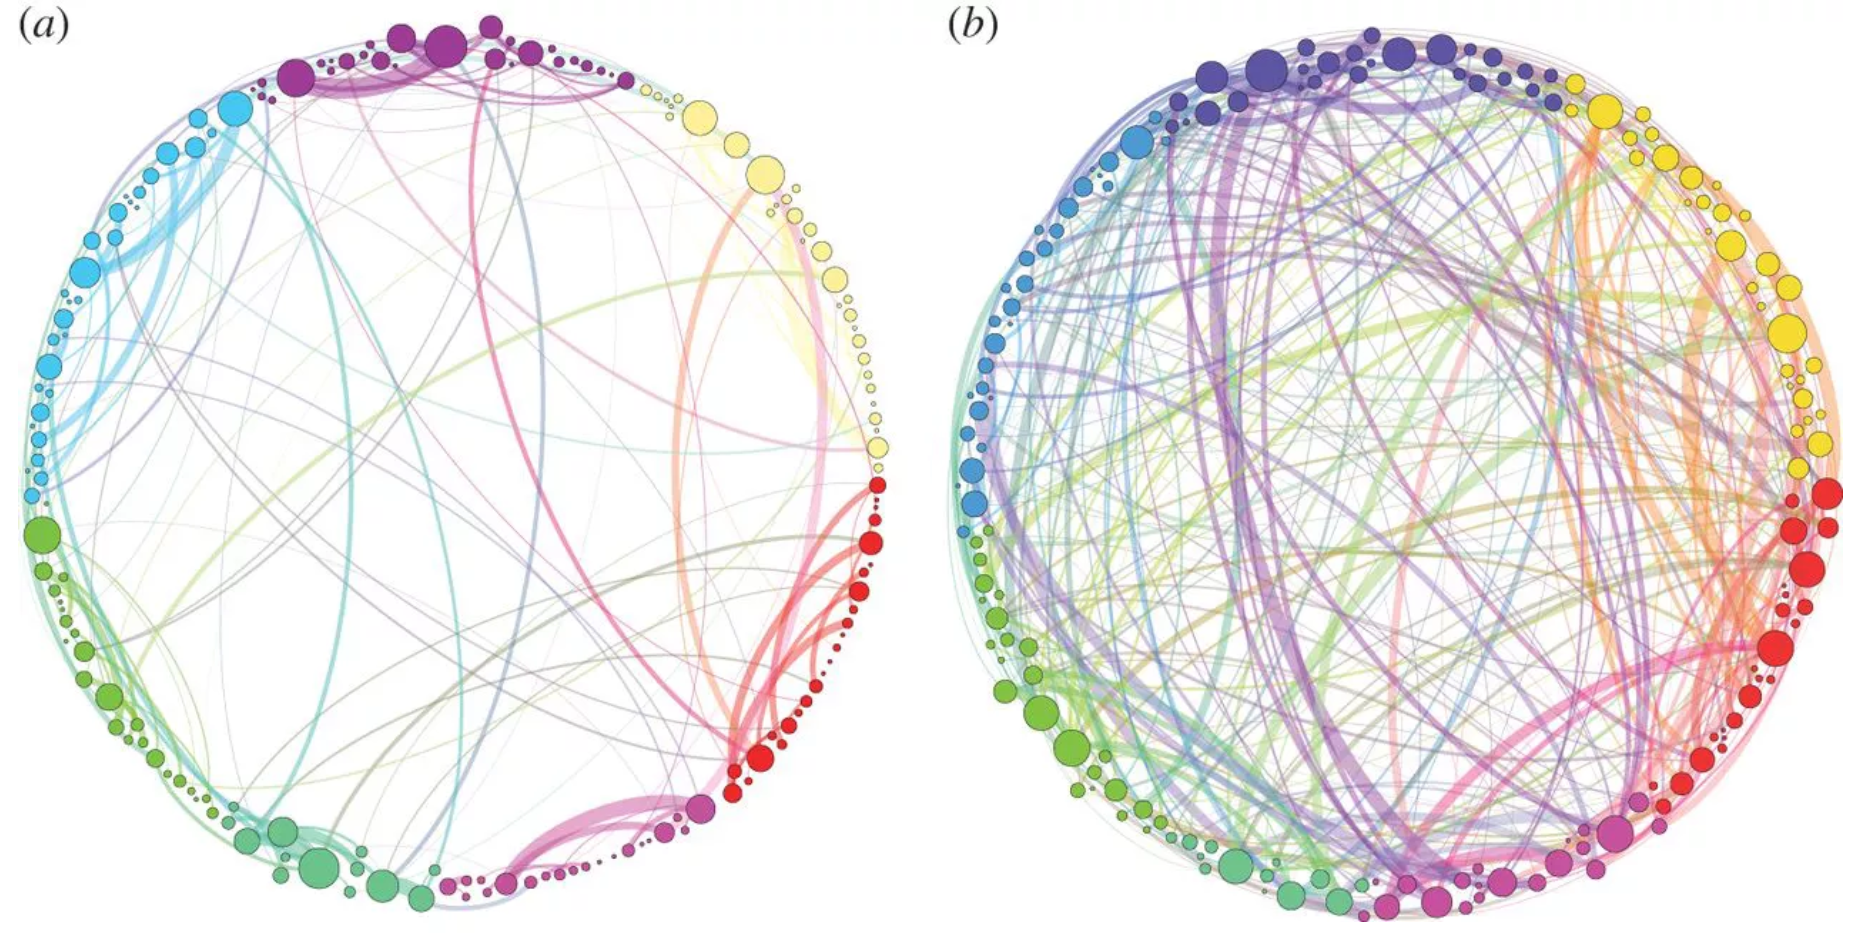
\includegraphics[width=\linewidth]{dmn.png}
	\caption{Brain activity measured by fMRI. In diagram (a) the subject using placebo. In diagram (b) the subject is using psilocybin}
	\label{fig:dmn}
\end{figure}

\subsection{best practices}

Eventually, in this reading, the elephant becomes too big for the room. The 1970 Controlled Substances Act became federal law, making illegal the possession and consumption of the classic psychedelics LSD, mescaline, and psilocybin. At the time of the law's passing 25 years had passed since Hofmann's fateful bicycle ride. The final 20 years had produced thousands of positive, scientifically valid reports, with ten's of thousands of human subjects high majority reporting positive reviews. Psychiatric research demonstrated positive unheard-of positive results in mentally ill and chemically addicted patients. Experiments in creative performance had provided strong evidence that psychedelics could lubricate insight, innovative thinking, and revelation.  

\subsection{third wave psychedelics}

\begin{snugshade*}
{Hofmann wrote a letter in 2007 to Jobs at the behest of his friend Rick Doblin, who runs MAPS [dedicated to studying the medical and psychiatric benefits of psychedelic drugs.]\\
Founded in 1986, the Multidisciplinary Association for Psychedelic Studies (MAPS) is a 501(c)(3) non-profit research and educational organization that develops medical, legal, and cultural contexts for people to benefit from the careful uses of psychedelics and marijuana.}\\
\emph{Healthy Normals}
\end{snugshade*}

\begin{quote}
\textit{{Dear Mr. Steve Jobs,\\
Hello from Albert Hofmann. I understand from media accounts that you feel LSD helped you creatively in your development of Apple computers and your personal spiritual quest. I'm interested in learning more about how LSD was useful to you.
I'm writing now, shortly after my 101st birthday, to request that you support Swiss psychiatrist Dr. Peter Gasser's proposed study of LSD-assisted psychotherapy in subjects with anxiety associated with life-threatening illness. This will become the first LSD-assisted psychotherapy study in over 35 years.
I hope you will help in the transformation of my problem child into a wonder child.\\
Sincerely,\\
A. Hofmann}}
\end{quote}

\begin{snugshade*}
- First reboot, 1995 Germany:
Mescaline-induced psychopathological, neuropsychological, and neurometabolic effects in normal subjects: experimental psychosis as a tool for psychiatric research.
\end{snugshade*}

\begin{snugshade*}
- 1996, US, Strassman DMT:
Human psychopharmacology of N,N-dimethyltryptamine
\end{snugshade*}



In April 2019, The Imperial College of London launched the world's first Centre for Psychedelic Research. Later that same year, Johns Hopkins University School of Medicine announced the opening of The Center for Psychedelic and Consciousness Research. In a statement issued by Roland Griffiths, the Hopkins center director and a professor of behavioral biology, \enquote{The center's establishment reflect a new era of research in therapeutics and the mind through studying this unique and remarkable class of pharmacological compounds.}

In both of these universities, as well as Harvard, Yale, University of New Mexico, and others, research on the effects of psychedelic drugs on the conscious have been quietly conducted since Rick Strassman's seminal study at the University of New Mexico in 1996, Human psychopharmacology of N,N-dimethyltryptamine. In the meantime, several formal groups, academic, non-profit, and even social collectives, have formed to support the continued study and therapy of altered psychedelic mental states.  Yale Psychedelic Science Group, Multidisciplinary Association for Psychedelic Studies  , the Portland Psychedelic Society, Toronto Psychedelic Society, just to name a few.

The Nielson Lab at the University of Minnesota conducts multidisciplinary research in the fields of neurobiology, psychiatry and informatics to treat trauma. Dr. Nielson's recent research into neurological mechanisms of altered states of consciousness and their role in promoting neuroplasticity and wellness in healthy subjects, funded in part by local community donations \cite{noauthor_nielson_nodate}. The network graph [see figure \ref{fig:therapy}] is a model of overlapping symptoms of trauma, and various psychedelic therapies that have published research suggesting a therapeutic benefit.

\begin{figure}
	\centering
	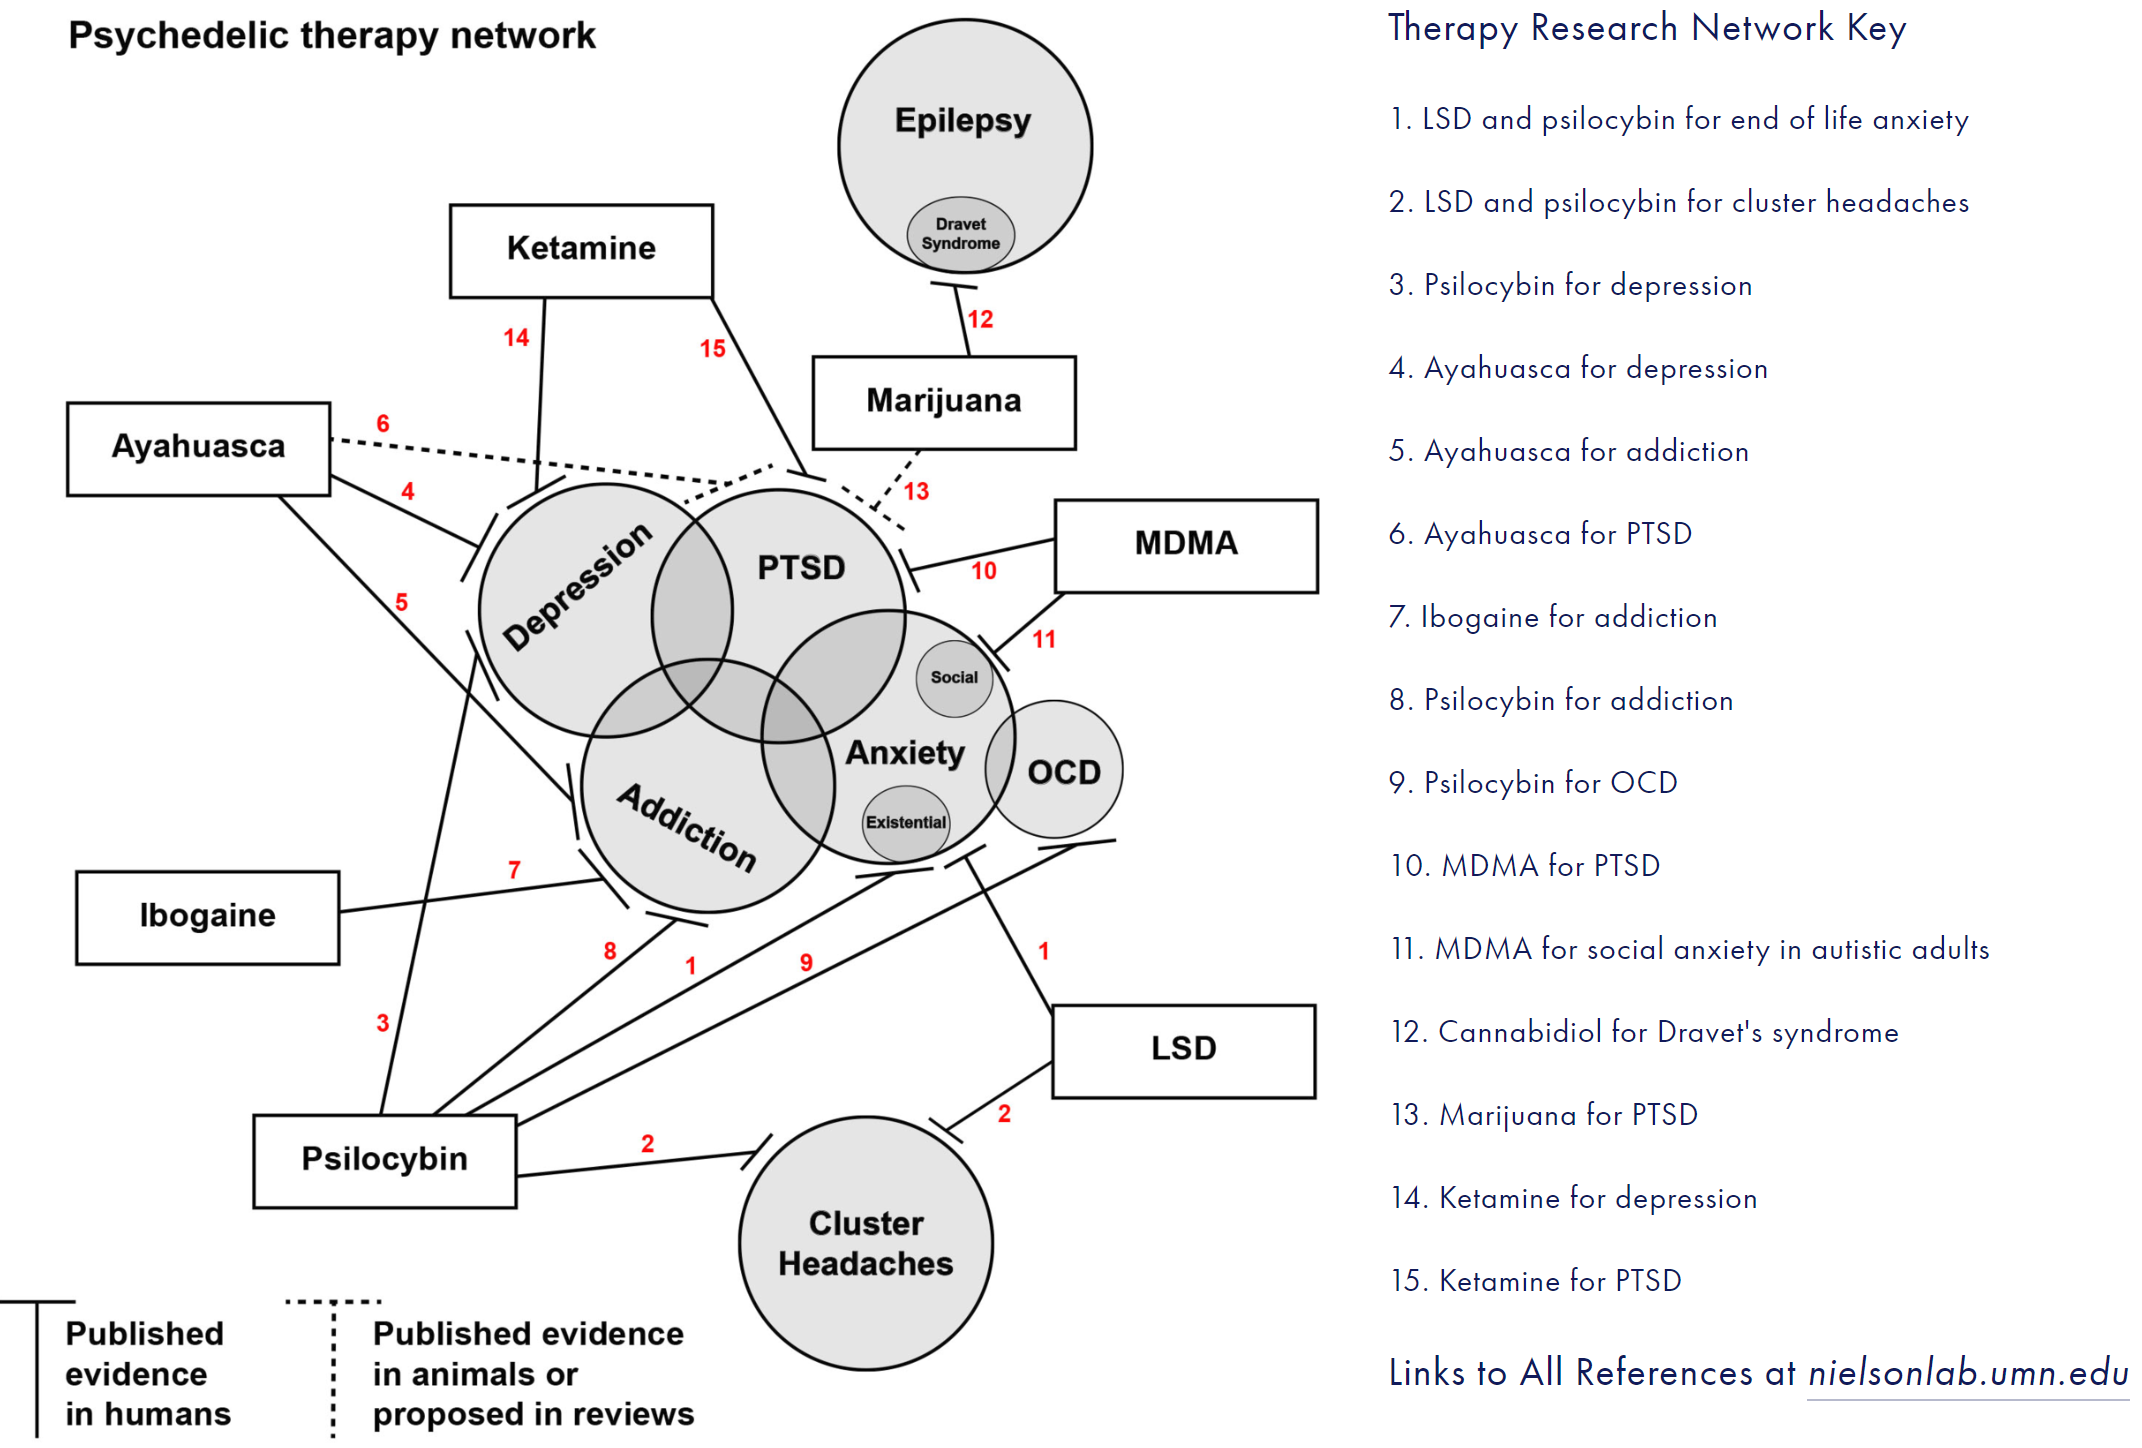
\includegraphics[width=\linewidth]{therapy.png}	
	\caption{Psychedelic Therapy Network diagram, Nielson Lab, University of Minnesota}
	\label{fig:therapy}
\end{figure}

Tolerance of psychedelics for treatment and personal development is leading to changes in both law enforcement and drug policy. In recent years, the California Institute of Integral Studies has offered a certificate program in Psychedelic-Assisted Therapies and Research. CIIS provides public education about psychedelic research and the use of psychedelics in psychotherapy, as well as teaching on topics such as creativity enhancement, consciousness studies, comparative mysticism, well-being enrichment and harm reduction \cite{noauthor_ciis_nodate}.

\clearpage


% --------------------------------------------------------------------------
% -- CHAP 3 --
\chapter{Crossing Reality}
\noindent
{%
\setlength{\fboxsep}{0pt}%
\setlength{\fboxrule}{1.5pt}%
\fbox{\includegraphics[width=\linewidth]{reality_head.png}}%
}%
\label{Chapter:CrossingReality}
\epigraph {You are the universe experiencing itself.}{Alan Watts}

\vspace{9mm}

It may be deduced that it is the interplay of Self-in-World, and the matter in which that relationship is observed via each observer's unique perspective, that leads to transcendent experiences. If this is so, is it also possible to direct the development of strictly external sensations to elicit similar outcomes? This paper explores the use of \textit{\ac{XR}} to craft uniquely adapted multi-sensory ecstatic experiences.

Cross reality is a technique that makes use of technologies of virtualization---sensory simulation of a believable world---and interaction with adaptive data processing, to include any accessible global data and real-time characteristics of the user. Unlike AR augmented reality, XR employs, among other features, a degree of artificial intelligence (AI). Objects in XR have adaptive routines---situational awareness. For example, an AR cat can sit on the floor, the dinner table, or in the center of your plate---it is ambivalent to its lack of decorum. If the cat were a denizen of the \ac{XR} universe, it might instead hack into your \textit{\ac{IoT}} doorbell to get you up from the dinner table so it can 'eat' your sushi while you are distracted.

The example seems perhaps glib but is never-the-less appropriate. Harnessing the potentially limitless data of the internet, distributed or \emph{edge computing}, and immersive human interface, \ac{XR} enables the technological animation of the environment as character. The state of technology today stands at the threshold of a new paradigm in shaping reality.


\section{Gathering the Senses}

\begin{quote}
{
\textit{Bounding through the world at a jog}, your bones register a rhythmic impact of earth against your form, while a concert of finely detailed muscular contractions press you forward with adaptive precision. Your heading brings updates, at 1000 times per second, the coherent light of the sun, pressed into the infinite reflections of every material existing beyond above and below, into a warm omni-directional ambient radiance--you can read even the shadow-side of every boulder, tree, and blade of grass. Your picture of the world, sweeping 180 degrees, bits of data concatenated from the buzz of 3 million excited nerve fibers crammed into an area 1/20th of 1\% of your body's surface area. For that report from the outside world to register anything beyond chaotic noise, fifty percent of your cortex is dedicated to processing visual information.

A vibration comes through the air, tunneling through first your right ear, then, with detectable distinction in time and tonality, your left. You deftly halt forward progress, crouching low in tall grasses, hand reflexively shifting to a throwing grip on the javelin. The acoustical pattern is familiar, and the method of the report tells you that a group of game fowl is stirring, probably just out of sight over the ridge to the right of your current heading. Are they aware of your presence as you are of theirs? Is their stirring a reaction to your disturbance, or some other third-body causality?

A breeze lifts tiny hairs on your arms, signaling a delicate shift in the non-corporeal medium of invisible fluid air, moving across this plane where your existence is registered. Like the acoustical signal, the passage of this movement also implies directionality, and without much conscious effort, a picture of the world becomes clearer. For the warm slanting rays of the Sun have dimmed perceptibly as you take in the scene, and combined with the sudden breeze, you know that night is mounting to draw a curtain across the sky, diminishing your effectiveness, and drive you to seek shelter.
 
But here and now, at this moment, your awareness reveals that you are downwind of the squawking animals, who, like so many other creatures, are entering an excited active phase, as the Sun dips toward the horizon. You know these wild turkeys will line up, and march with the Sun at their backs, in formation, rounding up insects from the waving grasses for a delicious snack. In moments, they will appear to you atop the hill.
}
\end{quote}
\section{Coding}

\epigraph{Information is just bits of data. Knowledge is putting them together. Wisdom is transcending them.}{Ram Dass}

Excluding periods of unconsciousness or trauma, most people have the perception of a reasonably continuous storyline without breaks and inconsistencies. Like a comet, details of the past fade to transparency, the further down the tail one traces from the present. 

Past experiences are more than just records of deeds and actions gone by; they are also filters to the present---providing an interpretation of our symbolic representation of the present and future.

This bias projection, or bias confirmation, is a vital component in delivering the conscious being's perseverant need for consistency

\clearpage

% --------------------------------------------------------------------------
% -- CHAP 3 --
\chapter{Building Reality}
\noindent
{%
\setlength{\fboxsep}{0pt}%
\setlength{\fboxrule}{1.5pt}%
\fbox{\includegraphics[width=\linewidth]{build_head.png}}%
}%
\label{Chapter:BuildingReality}
\epigraph {The mind is its own place, and in itself can make a heaven of hell, a hell of heaven\ldots}{John Milton, Paradise Lost}

\vspace{9mm}

The world perceived is a complex interaction of raw sensory stimuli and state of mind, referenced to personal experience through a time-based persistence. The resulting product is a subjective reality. As described in Best Practices, the features of \emph{Set} and \emph{Setting} are parameters that influence the resulting sense of \emph{what is real}.

Ecstasy is a process of experiencing exhilaration; a journey of heightened emotions and altered perceptions resulting in a reprieve from ordinary expectations. When considering feasible sources for ecstatic elevation, the catalysts of meditation and psychedelic mediation are, once `ingested', a function of physiology, and therefore, internalized processes. An ecstatic sojourner does not need sensation from eyes to `see.' Fully sighted persons can block all light from entering visual systems, thereby join blind persons in having wondrous visions \cite{sacks_hallucinations_2012}. Altered states perturb the sensations and perceptions of sensory data, even when there is none transducted from the expected channels to the outside world. However, physical senses should not be discounted. What happens if the world sensations are \emph{altered} before	they emanate from the `real world?'

Within the technology of \textit{\ac{XR}} lies an opportunity for refined influence on set and setting. Contemporary technologies of virtual world-building place fine-tuned controlled of an immersive sensory setting in easy reach, and the adaptive intelligence promised in deep learning emboldens features of the perceived world into conscious character. Conceiving of technique that enables real-time phenomenal hallucinations is not far-fetched. Here we postulate it is possible to use the technology of XR to elicit an ecstatic response---from the outside in.
 
\textit{\ac{EXR}} offers hitherto unreachable features of altered state consciousness. Chief among them is the opportunity to be observed by third parties---which is to say, empirical, and to some degree, reproducible. \ac{EXR} can be simultaneously a door to deep personal discovery, and a research tool into the workings of the conscious mind.


\section{Ecstatic Simulation}

Since time immemorial, humans have been using representational imagery to explain personal experiences, to record events, and to communicate ideas. Although art for art's sake is not to be diminished, the power of symbols as a tool for elevating understanding and advancing abstract thinking is undeniable.

Archaeological discoveries reveal that prehistoric peoples have sought to represent the occurrences of ecstatic altered states. As the collective skill in artistic representation and the technological refinement in the variety of media tools advanced throughout the ages, the ability for image rendering steadily increased to a degree of complete realism. By the time of the Renaissance, the mastery of perspective technique with the versatility of oil painting, and an exquisite understanding of human physiology, it became second nature to craft evocative single-frame stories in painting, sculpture and fresco, depicting either real or imagined compositions of great significance.  

With the perfection of representational art achieved, the subsequent art movements of impressionism, surrealism, cubism, and the entire range of symbolic deconstruction beginning in the \nth{19} century, were possibly a logic anecdote for the shackles of reality. Salvador Dali created compositions that were at once completely real in form, yet wholly fantastic in set and setting.

Once the technology of art allowed for altering representation in time, with sequential imagery, filmmakers had access to storyline in four dimensions. Now that producing 4-dimensional media is child's play, a global internet pushes HD quality video into every hand that beckons. That on-demand media has a measurable impact on the way reality is rendered moment-to-moment in the industrialized world, is not a hard concept to grasp. Henceforth, we are immersed.
Considering humanity's enthusiasm for representational art, and the provocative influence of ecstatic altered state consciousness, it is not surprising that there is a considerable body of \emph{visionary art} to be found. Putting conventional tools of the \nth{20} century to the task, it is inevitable that a majority of ecstatic art follows a one-way, methodical \emph{formulaic} process. 


\subsection{formulaic}

Formulaic artforms are processes wherein the resulting forms are established and bound by selected input parameters. While it is not possible for a painting, or a musical score, or television show to program everything about a viewer's experience, it is practical to suggest that the media presents its content at the surface, without input from the audience. The result is unidirectional; no dialog is taking place, even if the audience is eager to comment.
Formulaic ecstatic art can be \emph{linear} or \emph{parametric}.

\subsection*{\ldots linear}

Linear artforms are bound by the direct manipulation of medium in time. The parameters for input are frozen in the result, creating an indelible product. There is one direction forward in the creation of the work, and all manipulations are found in the minds of the creators, regardless of the kind of editing tools the medium uses. For example, painting on a canvas with oil paints allows editing in physical layers, through the process of time. One could philosophize the work is composed of layers of time, as equally as layers of paint. Only one painting exists at any time, and perhaps the artist will proclaim it complete at some arbitrary phase. 

Sequential art is a linear art form as well, as long as the parameters for creating it are, again, composed in the minds of the makers, using the tools of the media directly. In this case, lighting, lenses, light-sensitive medium. Even a computer using non-linear editing software for adjusting the sequence of frames. The resulting video is a linear product, with one expressed intention for reading its message.

Ecstatic art in linear mediums such as these are snapshot emulations of conceived altered mind states. Representing the features of altered reality, the tools of linear art are transformations of space, scale, perspective, and time. They can be ``trippy'' and evocative, even reminiscent of an audience's recollections, but they are not likely to legitimately trigger a uniquely ecstatic voyage on there own.  

In the static frame image genre, artists like Alex Gray, Michael Divine, and Android Jones depict transpersonal ecstatic moments in third person surreal imagery. The impact of moving pictures can be considered in films like Enter the Void, a 2-hour film released in 2009 depicting a real-time first-person DMT trip, followed by the remaining screen time experienced as a pseudo-second-person after-life.

Whether these works are an attempt to recreate, symbolize, or broadly make commentary about psychedelic mind states, it is unlikely that any strictly sober, beta-wave conscious viewer will ascend into an expanded consciousness simply by viewing these media.

\subsection*{\ldots parametric}

Whereas linear art forms are created, on the whole, by accumulations of manipulation by the artist, parametric artforms harness the logic of iterative transformation. For practical discussion, this method relies on the input of computer-mediated or computer-controlled parameters, and as such, harness a conscious or quasi-conscious sensitivity beyond the purview of the artist alone. 

Parameters can be algorithmic, meaning objectively mathematical, programmed into the matrices of the solution. For example, algorithmically-driven art can explore the fractal visual routines embedded in a single formula. Consider the variations on Mandelbrot zoom easily searchable on the internet, which rely on the following math to plot a graph on a time-base index: 

\verb|[f[{a_, b_}] := {a*a - b*b + c1, 2*a*b + c2}]|

This fractal was first defined and drawn in 1978 by Robert W. Brooks and Peter Matelski, and first visualized by IBM in 1980 \cite{taylor2008biophilic}

If the series of still frames shown in figure \ref{fig:mandel} fail to impress the reader, try instead a 70 minute colorized 4K dive at 60 frames per second. It may not be ecstasy inducing, but it is nevertheless quite mesmerizing \cite{noauthor_eye_nodate}.

Fractal math can be impressive, but after showing its hand, the mysteries are diminished. The results are restricted by the formula, despite the variation in stylings chosen by the artist. Computer music visualizers can play with parameter-controlled visualizations using the music source as a constantly variable seed. This has the additional effect of allowing a listener to `see the music,' a reasonable variation on the theme of synesthesia.
 
Pushing the concept a bit further, the process can be augmented further by the additional interjections of neural network processing. In this case, the mathematical framework allows for concurrent computational parameterization at the time of frame processing. Google's Deep Dream is one example. Start with a \emph{seed} image, add one or more influencing style image, adjust the variety of parameter sliders, and send the package off to Google's deep neural network to generate a result. No two results will be alike, even if the same package is submitted repeatedly. The iteration parameter determines how many loops to iterate over the final frame, resampling the frame before declaring a result. The more iterations, the more altered the seed image becomes. Using Deep Dream to produce a sequence with a zoom such as used in the Mandelbrot set, will produce a very compelling hallucination, indeed. 

Techniques like this invoke many nomenclatures, but the general process is called deep learning, or machine learning, and is a foundational feature of artificial intelligence. In this case, Google's Deep Dream is programmed to nudge successive images slowly toward biased outcomes, namely, faces, animals, buildings and landscapes. 

Another machine learning system invented by Ian Goodfellow in 2014, known as \textit{\ac{GAN}}, comprises two neural networks contesting with each other in a game. \acp{GAN} have been trained to produce extremely believable `photographs' of human faces. The open-source project, CycleGAN, initiated by Jun-Yan Zhu of Adobe research, demonstrates an image translation implementation able to use video of a dramatically moving horse, taken from a moving camera, with both foreground, middle ground, and background elements, and track very believable zebra texture mapping onto the horse's apparent topography. If a friend claimed that the obvious quarter horse in the pasture in front of you was clearly a zebra, you might wonder if something funny got into her tea [figure \ref{fig:gan}].

\newpage
\begin{figure}[h!]
	\centering
	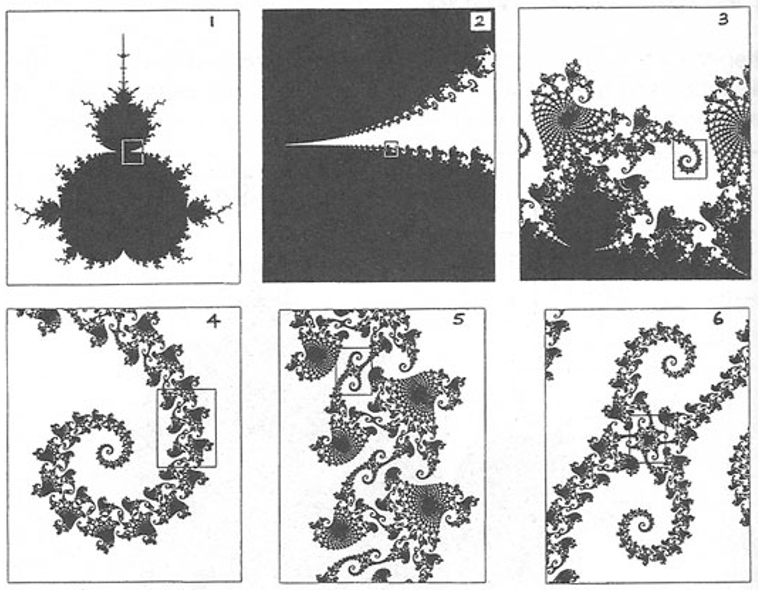
\includegraphics[width=.81\linewidth]{mandel.png}
	\caption{Scale zoom on fractal Mandelbrot set. Infinite iterative transformation}
	\label{fig:mandel}
\end{figure}

\begin{figure}[h!]
  \centering
  \begin{subfigure}[b]{0.4\linewidth}
    
\includegraphics[width=\linewidth]{predeep.jpg}
    \caption{Original image}
  \end{subfigure}
  \begin{subfigure}[b]{0.4\linewidth}
    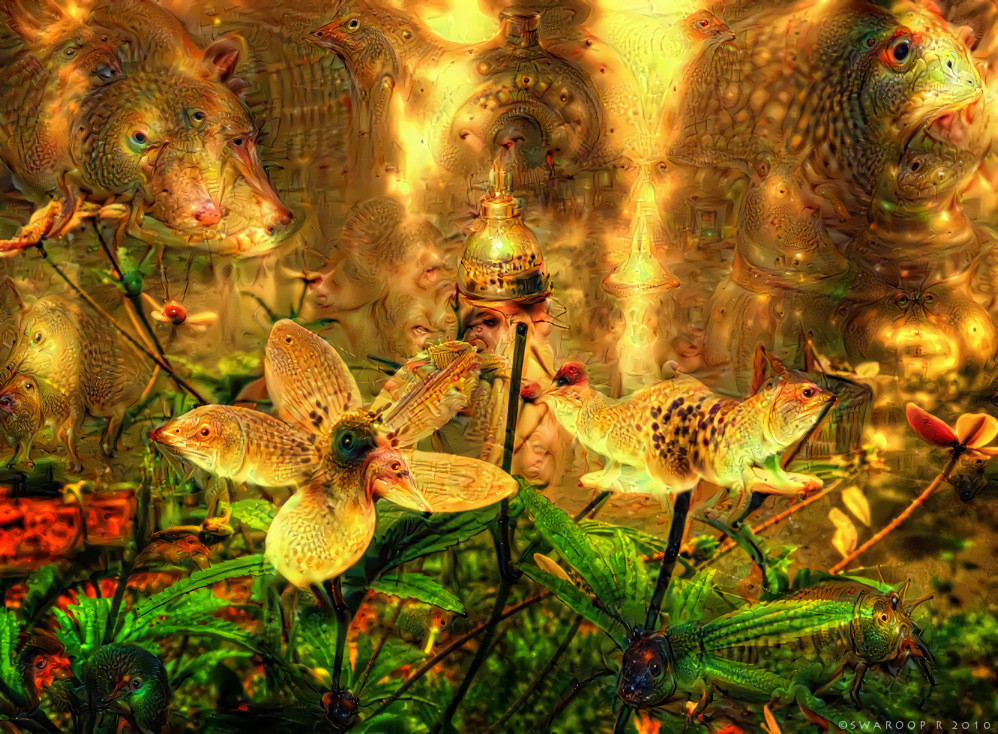
\includegraphics[width=\linewidth]{deep.jpg}
    \caption{Google Deep Dream}
  \end{subfigure}
  \caption{Neural network iterative image processing}
  \label{fig:deep}
\end{figure}

\begin{figure}[h!]
	\centering
	
\includegraphics[width=0.81\linewidth]{gan.png}
	\caption{horse to zebra, original frame and manipulated frame, CycleGAN on Github}
	\label{fig:gan}
\end{figure}

\begin{figure}[h!]
	\centering
	
\includegraphics[width=0.81\linewidth]{gan.png}
	\caption{horse to zebra, original frame and manipulated frame, CycleGAN on Github}
	\label{fig:gan}
\end{figure}


\section{EXR}

For thousands of years, humans have been augmenting the perceived story of existence via ever more complex technical mediations. Since the beginning of the \nth{20} century, artists have utilized recorded sounds and visual apparitions to create ever more immersive pseudo-realities for entertainment, communication and learning. Filmmakers often refer to the \emph{suspension of disbelief} as a key willing involvement between media and the consumer. 

Providing interactive input between users and the media enhances the sense of immersion for participants. Interactivity requires the use of a device. Humans, being tool users, and adepts in symbolic abstraction, easily incorporate language and props as triggers and game pieces. The audience can break the fourth wall with actors or quasi-sentient characters to become full participants in a kind of gameplay. Keeping in mind that consensual social rules are also devices, the material, social realm demonstrates this daily; people scramble for resources [on all sides of the rules] in the cultural game of living.

Without becoming too esoteric, let us refocus on the topic at hand: XR and the inorganic physical device that comprises a human-computer interface. At the time of this writing, consumer-grade virtual reality devices are widely accessible. The hardware has rapidly improved in terms of image quality and speed, as well as becoming less bulky, more comfortably fit, and more affordable.

Activating \ac{XR} does not have to mean strapping on an array of devices. For the time being, however, the developers' platform is ready for implementation in this format.

In the previous section, ecstatic art forms were relegated to a formulaic producer/consumer approach. That is to say, the audience does not partake in the visions, she merely receives them and makes of them in their form what she will. EXR makes additional advances in ecstatic narrative in the following ways:

\begin{itemize}
  \item Rendering the perceiver's perspective adaptively, in real-time
  \item Providing input control with feedback
  \item	Access to unbounded data 
\end{itemize}

\subsection{perspective}

People are accustomed to their biological sensor arrays as currently situated with respects to their bodies. They are remarkably capable of negotiating a complex shifting built environment, without injury or loss of continuity. A healthy human can find her left big toe in the complete dark within seconds of waking up. She can walk backward into her apartment pushing the door open with one foot while her arms are encumbered with shifting centers of gravity in multiple groceries bags. During the first visit to her mother's new house, at 20 paces, she can recognize a 30-year-old photo of her childhood pet attached to the refrigerator with a circular magnet and remove it with two fingers without interrupting a conversation with her insurance agent on the cellphone pinched between her cheek and shoulder.

It takes a powerful mediation to break that kind of hold on `reality.' There is little wonder as to why ``trippy visions'' and deeply mystical experiences are easily dismissed as nutty aberrations when they are not personal. Our senses of the real world are phenomenological. To convincingly mediate a viewer's reality, using the complete array of senses will be the most effective.

The ordinary VR headset is remarkably good at this. Just taking the visual headset alone, without any audio or tactical input/output [which is currently very course], the position of the viewer's body transforms the virtual camera's view into the virtual world. This delivers a convincing sense to the viewer that she `is there.'

\subsection{controls}

The most provocative and natural input control for the EXR platform is the user's body. Human beings spend the first [three] years of their existence programming their nervous systems to process sensory data and manipulate their physical housings, navigating complex space, and time. 

The visual system dominates human sensory processing. A majority of the cortex is dedicated to handling sensory stimulus input from the eyes. Fortunately for the EXR premise, screen technology has made huge leaps in resolution, fidelity, and has multiple solutions, from lasers, OLED, LCD, bistables (electronic ink), and so on.

One dramatic weakness for input/output systems in current technology is in haptics, or tactile, feedback. The human proprioceptive sense is also taken for granted. Notable in the report of ecstatic experience, is whole-body physiological response. A very compelling EXR simulation would benefit from immensely from tapping into that landscape. 

In the present era, developments for more sophisticated and wider bandwidth controls are envisioned or under literal development. The leading \textit{\ac{BMI}} peripheral is Elon Musk's Neuralink. The device makes use of cortical implant technology to insert arrays of electrodes \SI{5}{\micro\meter} in width and numbering up to 3,072 electrodes per array. 


\subsection{data}

As expected, EXR makes use of all the features of a connected world. Whether a future generation of wireless, or minimally-tethered, the compute demands for a responsive and aware sensory simulator will be considerable. Accessing parallel computing in a local network, or the cloud, with historic user profile-based machine learning will be essential. \emph{Edge computing }is a current term that captures the demand cycle transport of I/O for connected devices in the current buzz lingo of disruptive tech.

To create a believable personalized immersion and break into the world of ecstasy, an ecstatic cross reality platform will be aware of the user's biometrics and brainwaves. Eye movements, respiration, and pulse are high-value inputs. \textit{\ac{EEG}} or similar conceptual \ac{BMI} like Neuralink would enable advanced responses and awareness.

\section{Ecstatic Mediations}

As with any good design, technical gimmicks and creative aspirations are only as good as the execution. Buster Keaton was able to make people shriek and duck in terror in the primitive, soundless theaters of the early \nth{20} century. \ac{XR} technology is in a comparably similar phase of development. For examples of what might be possible in transpersonal \ac{XR}, consider the work in \ac{VR} by Sander Bos in which live music from a sitar, flute and hang drum transform elements in real-time visualization. In the virtual world, a glowing aura-enshrouded sitar player seems to occupy the place where the music emanates from in the real-world room. Landscape elements shift and move, as the viewer's perspective shifts and transforms, creating an apparent movement [still frame shown in figure \ref{fig:bos}].

View the video recording captured at a demonstration in Groenigen in 2016 \cite{noauthor_raga_nodate}.

\begin{figure}[h!]
	\centering
	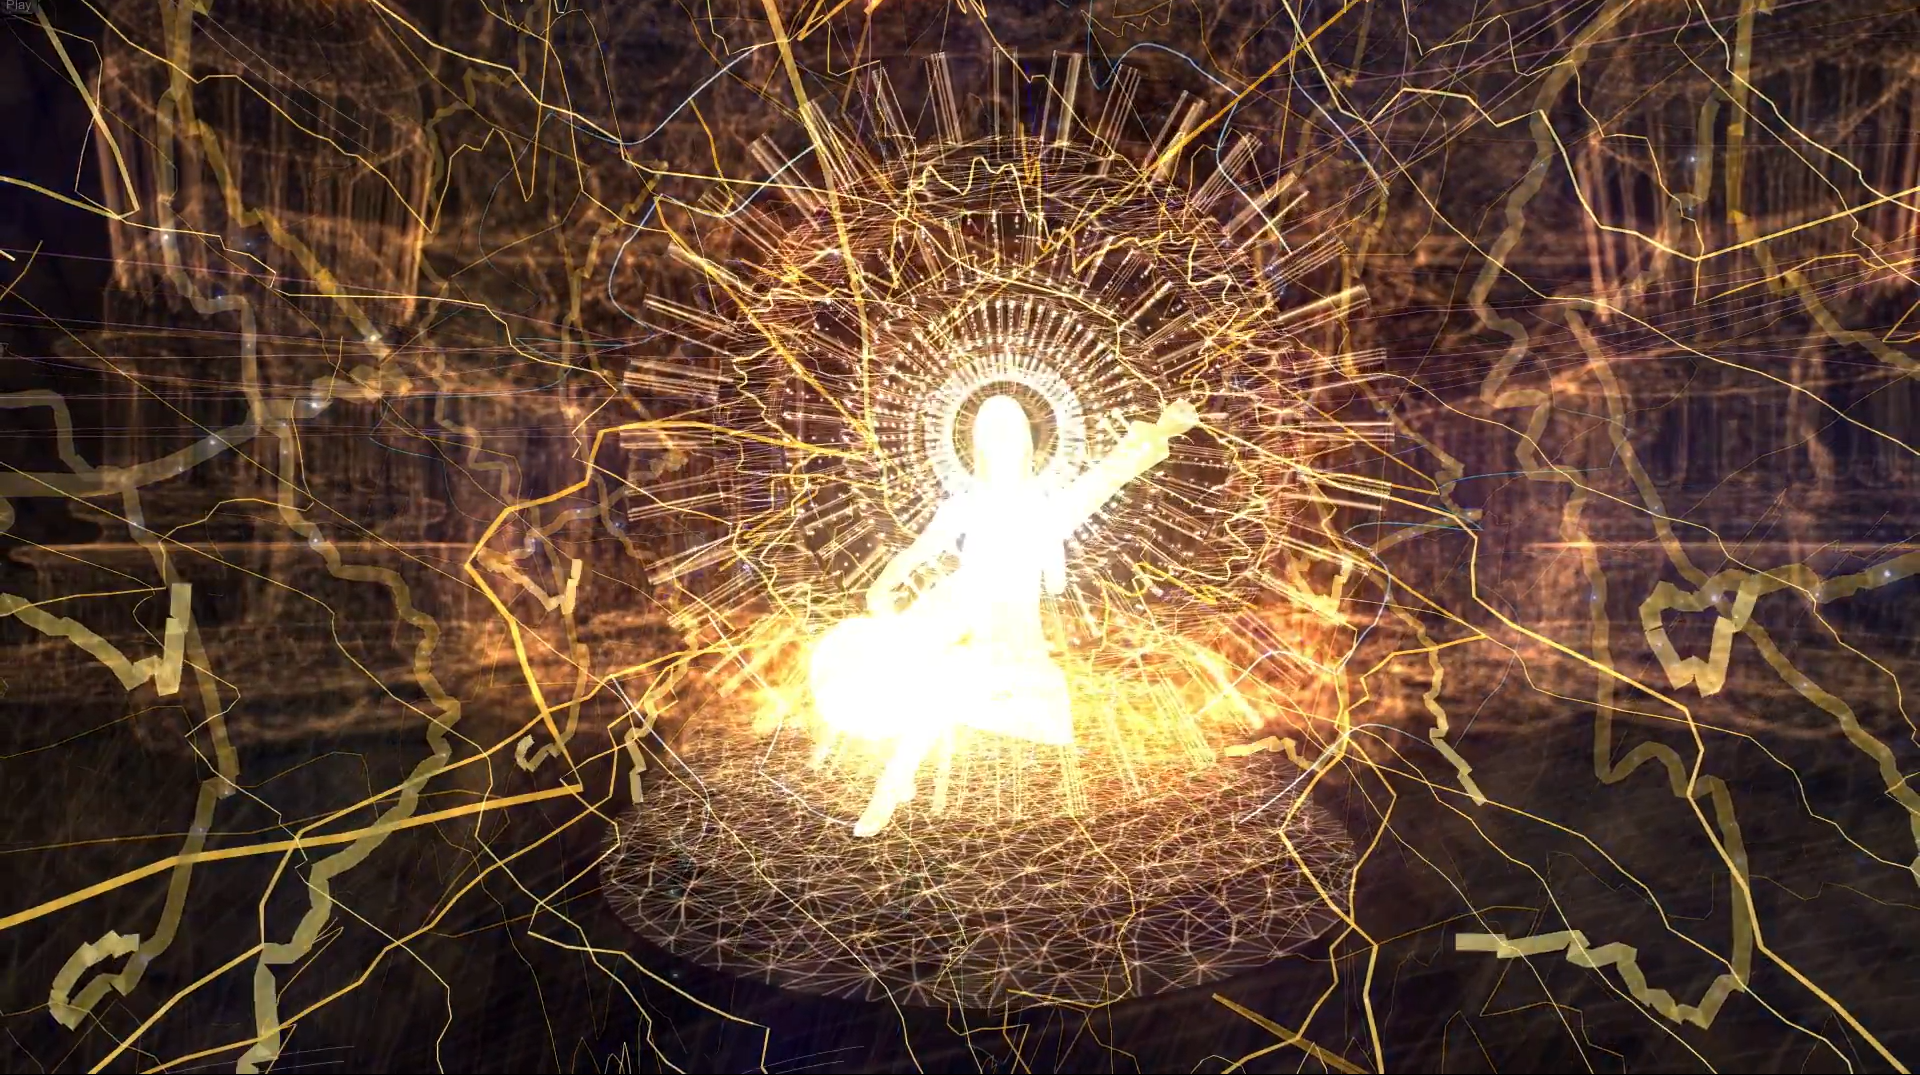
\includegraphics[width=0.81\linewidth]{bos.png}
	\caption{Raga Chromesthesia, Sander Bos 2016}
	\label{fig:bos}
\end{figure}

\subsection{psychotherapy}

In a relatively obscure online podcast tilted, Psychotropic: stories involving psychotropic drugs, is the story of Jesse, a young graduate suffering depression and anxiety from a long-time repressed childhood trauma. Without professional help or diagnosis, he experimented with mushrooms and DMT, resolving to self-prescribe combinations of daily meditation, and occasional psilocybin to maintain a positive mood. Jesse judges the therapy successful and further engages a professional psychotherapist who practices \textit{\ac{EMDR}} therapy. 

\ac{EMDR} is accepted as an effective treatment modality in Cognitive Processing Therapy by the American Psychiatric Association, developed in the 1990s. The distinguishing mechanism of \ac{EMDR} involves guided sessions wherein the administering therapist works through traumatic events by asking patients to recall distressing images while stimulating them with some form of bilateral sensory input---alternating bilateral sensation, by periodic switching between brain hemispheres, via lateralized sensory processing. Common methods are to request the subject to follow a pendulum focal point with only their eyes, which could be the therapist's finger, an oscillating light, or the like. The electronics marketplace being what it is, \ac{EMDR} kits comprised of a wide focusing light bar, headphones, hand-held vibrating pucks, and a controlling mobile application, are easy to buy online. 

If this sounds a bit like a technique of \nth{18} century hypnotism---a medallion putting a subject into a trance---Jesse might agree, as he insists that the process helped him to deal with undesirable thoughts by encouraging disassociation, enabling him to \enquote{\ldots[access] harder memories that are more difficult\ldots kinda like psychedelics. When I take mushrooms, it's similar.}

An early field test to evaluate the effectiveness of EMDR therapy, sponsored by the VA Mecial Hospital and Colorado School of Professional Psychology, was trialed in the immediate aftermath of the 2001 New York 9/11 attacks. The study relied on local EMDR certified therapists providing up to five pro bono sessions to treat a cohort of 65 subjects drawn from populations directly impacted by the World Trade Center disaster. 

The study made two conclusions. First, that simply EMDR is a useful treatment intervention in the immediate aftermath of a disaster. Secondly, psychological treatment in mass disasters is often complicated by the suddenly unfavorable ratio of patients to available therapists. The sheer number of clients, the turmoil of movement in the lives of the families of the survivors, and the general downstream mayhem can harry effective scheduling. For example, in the initial screening, 141 individuals contacted the emergency network for candidacy, but over half were eliminated for staffing limitations or were unable to complete all the sessions.

Here is an opportunity for augmenting the aforementioned ``EMDR kit'' with the features of a customized EXR.

Theorizing about the features of an EXR EMDR platform, the task of delivering bilateral sensory input is inconsequential. Consumer-grade VR platforms of today can easily direct stereo visual and audio with perfect precision. Haptic feedback, although limited, also ships standard with a complete commercial package. As the visual and audio stimulation is highly configurable, with HD quality moving images delivered to the eyes and full frequency response to the ears, the possibilities for a sophisticated customized therapeutic session, are rich. A team of therapists could develop an online program using in-processing profile interviews, and passive progress monitoring from session data, without necessitating regular clinic visits or house calls. Patients and therapists can regularly tweak the profiles, configuring for other issues that unearth from the past, or develop in the present.

Such a system could conceivably multiply not only the effectiveness but the through-put of a wider therapy network. But why stop there? Customizing individualized sessions could expand in scope to include daily sessions for a broader population, following the progress of mediation applications and mindfulness techniques that show growing popular support in a stressed-out 21st century. Perhaps in time, as hardware evolves, especially input/output, an open-source configurable EXR therapy system could be trained into guiding a devotee into legitimate dial-up ecstatic bliss

XR could be applied to other psychological disorders such as depression, where one could develop empathy for themselves or anti-social disorders where they cultivate empathy for others.

\subsection{psychonaut}

\begin{quote}
{
I landed in a crouch, touching the ground in four points. Six points. I have two sets of arms, obviously.

Quarter-second tracers.

\textit{Phwooosssh!}

A burst of fragrant air blows against my face. I imagine tendrils of hair whipping behind me in slow motion. That lasted too long. It also happened too slowly---after my forward motion halted. Funny delay, that.

I close my eyes, throw my head back, and Ahhhhhhhhhhhh!! a full-throated baritone. Harmonics converge in impossible chorus on my head area. Acoustic wave-forms flicker in brilliant blue fire within my peripheral vision. My peripheral vision must be in some new dimension because my forward vision is a 360-degree fish-eye. When I want it to be.
\\*
Now, I don't. I need to rest. Darkness.

\textit{Sukhasana}. Deep slow breath.

My moments-ago sighing chorus with myself attracted giggling sopranos. Faeries again. I banish them with a huff. Delicate glass shatters, a short-lived local rainstorm. Tennessee Williams, Rain Menagerie. ``Rise and shine!'' Don't be ridiculous.

Let's start over.\\

Deep Slow Breath\ldots Deep Slow Breath\ldots \\
Deep\ldots \\
Slow\ldots \\
\ldots this could take awhile, why don't you come back?

\noindent\rule{2cm}{0.4pt}


The point of light is growing. Centered.

It is\ldots a golden\ldots geometrics. Why do six sides always dominate? Benzine rings, right? I gotta remember to ask Bucky. The bees know. Oh yeah, that's righ\ldots tubes just do that when you pack them together. I love that. Well it has to be something, you know? Why not hexagons.

Ok, pay attention. All these tubes are making a picture now.

If increasing resolution in a plane multiplies in squares, then it cubes with depth. It's just weird to think of the world as the sum of cubes. Yeah, voxels, whatever, no one says that anymore. Regardless\ldots we need to get bigger than that if we want to complete this visit.

``This way. Quietly,'' my dead cat says to me, looking backward over his shoulder as he eases forward through the tall savanna grasses. Sure smells nice here.

Smiling, I throw him a little nod and wink, setting my right paw down in the spot his rear foot just vacated. Following too closely, I think. Ok, I don't really want to be looking at your butthole, Jem. I chuckle.

Snap! I reposition off his left flank.\\
Snap! We crested a small ridge.\\

Looking into a tidy, colorful valley. Poppies, orange, dense, like the Antelope Valley. There. Are. No. Antelope. It's just a name.

There. Are. Butterflies.

``So, this is what you've been up to?''\\
``Yep,'' his toothy grin. His face looks Cheshire. It's a good fit. I think you could have used this face when you were alive. ``Ha! I did! You don't know everything.'' How true. How true.

We tense our leg muscles. We do that cat-haunch-wiggle-prepare-to-pounce dance. It feels good! I feel the charge well up from within, then spread outward, like pulling a blanket one cell thick across the surface of my skin; every cell tingles and bursts in a sequential crescendo.

We're off! I delight in the sensation as we bound down the hill and tumble in butterflies.

For eons. 

\noindent\rule{2cm}{0.4pt}\\
With an arc of saline fluid streaming from my arm, I sit up, wave my hand over the sensor glass to end the program. The dermal patch is hot and itchy on the back of my head. I feel around the unfamiliar mechanism, disconnect the fiber feed and gingerly tug the patch off. Remove the two Velcro ulnar bracelets. Meanwhile, gentle spotlights have come on, casting caustic reflections on the chamber walls from all this sudden movement in the water. I sit for some time, so the patterns can relax, too.
With a tight smile, and one more little nod to where Jem stood for that moment before the hunt, I rise from the tank, and reach for my towel.
}
\end{quote}
% --------------------------------------------------------------------------
% -- Summary and Conclusions --
\chapter{Summary and Conclusions}
\label{Chapter:SummaryAndConclusions}

% You can refer to chapters and sections using their label, e.g Chapter \ref{Chapter:Introduction}.

Born in the early 70s, I was fated to enter adolescence with Nancy Reagan's posters on the back of every homeroom door and those impressive adverts on television---about making breakfast in the frying pan? Maybe you know them. I remember, still, succinctly, my \nth{2} grade teacher proselytizing, \enquote{Just one fly's footprint of LSD can scramble your brain.}

I believed every word. I'm not sure if the messages were effective because of childhood gullibility, or a result of the ambivalence toward drugs after balancing risk versus reward. For \emph{what could be the reward?} I could not imagine. In the meantime, drug education in the 80s lumped every unsanctioned chemical into one category: narcotics. Narcotics users were desperate losers with debilitating tragic lives. They walked the line of addiction and criminal incarceration. None for me, thanks. I had no interest in any of it---not pot, not alcohol, not tobacco.

Alcohol is one such substance well integrated into our culture, despite the fallacious attempt to embargo it 50 years before I was alive. There may be government restrictions on marketing and distribution, but it was clear that some people could use it without disastrous consequences. And yet, abuse and addiction were still visible with this ``permissible'' substance.

Contradictions abound, right at the surface, and a critical mind will eventually resolve to provide custom guidelines for navigating the world of intoxicating substances as an adult. The first distinction that became clear to me, with nearly passive awareness, was the emerging difference between true narcotics and hallucinogens. I never once heard of a substance abuse center for magic mushroom addicts. Homeless LSD junkies? That's not a trope. I didn't socialize with drug-users, so I was not directly party to the features of the supply chain, but even in the pervasive anti-drug media narratives, there were no psychedelic school-yard pushers, no king-pin LSD drug lords. Miami Vice had cool heroic drug-busting cops---they took down cocaine and heroin rings, not Peyote button wizards, or weirdos licking Sonora desert toads.

That disparity reveals another clue to the discerning skeptic. The classical psychedelics are, technically, more restricted than the substances that the drug empires and the law enforcement agencies draw their power from. Considering this, and noticing that there are substantially fewer criminal events with psychedelics, raises a flag. While it is true that marijuana has an unfortunate history of cops and cartels, fortune and fatalities (cannabis needs its own story), it is otherwise the coke, heroin and illicit pills that bring in the Benjamins. It turns out that the classical psychedelics have a distinct consumer advantage over other drugs in their dose and exposure demand---a threshold experience requires minuscule dosage, and most users are in no rush to re-up. In the end, perhaps there is simply not much money to be made, so the concentration of power is minimal. For the true narcotics, the profitability is enormous, and the push-pull narrative of destruction following the illegal drug trade is legendary.
 
The initial investigating of this thesis centered on \emph{altered states}. I expected to hypothesize on innovations in consciousness, the inspirations found in a fanciful mind temporarily re-tuned. Key to unlocking that experience, I believed, was the temporary break from the persistent symbolic lock of momentary living. Every moment of consciousness is enthralled with the conformity of expectation. Imagine any day in life and the continuous conviction of abstract symbology that makes every particle of awareness rational. My responsibilities, my clothes, this table, food on a plate, vehicular traffic, images on screens, a flowering tree, financial obligation, my name--there's little break from any of it. The occasional mystery is given idle curiosity, (and might even become the subject of a quest to eliminate it!) until the pressure of some other duty closes the window. Those among us who don't behave with this kind of consistent acceptance (``\ldots you see little green men, you say?'') are often held to be a bit strange, or maybe even crazy, as people do suffer affective mental disorders that prevent so-called ``normal'' summation of all these interference patterns at any given moment.

To this end, I was inclined to model the reference disruption experience on psychedelics for their incomparable power to safely and temporarily shake up the snow globe. That seed idea offered three conceptual challenges, Condition A) what is this ``temporary insanity'' condition? What should I call it? The research needs a title, and I hoped to make it short and catchy. Condition B) What other methods or techniques would enable this mind state? Could not a disciplined mind break mundane reality? Congenital malformation, or brain injury? And Condition C) can the state be triggered, guided, or enhanced with ``virtual reality?''
The goal was to link altered mind states akin to psychedelic vision to the interface of virtual reality in a practical way. As an engineer/artist, the salient features would be not only practical, but aesthetic; theoretically feasible, and conceivably enlightening. I had doubts, but my major professor, no slouch in the fields of psychology and human-computer interface, urged me on.

Breaking the inquiry into the three sub-questions helped me to reduce the complexity and make sectional progress. Throughout the process, cumulative discoveries refined the underlying concept, often enabling settling across the triad relationship.

Discussion of psychedelic drugs brings with it the bias of taboo and legal consternation. Hoping to distance the writing from such prejudice, I discovered early on that the first serious researchers sought similarly to distinguish the character of psychoactive mind-expansive inquiry from the frivolity of recreation. Wasson, Ott and a small cohort gathered to discuss, and the term \emph{entheogen} emerged as their solution (Wasson, Ott 1979). For awhile, that was a focus term, and I attempted to lens the entire concept with it, but it did not fit well. Simultaneously, it made a bad title. 

After some discoveries, ecstasy became the focal term to encapsulate altered states of mind, Condition A, and as soon as I fully understand what it can mean, it quickly unearthed deep and well-documented association with meditation, religious revelation, and even psychotic illness. Throughout the scientific revolution, long before laboratory chemistry and the awareness of neurochemicals, philosophers of mind have observed the effects of ecstasy. Pre-enlightenment theologians write of ecstasy. Moreover, archaeological evidence has uncovered ceremonial practices, in art and burial ritual, that make a strong correlation to mystical occurrences, sometimes accompanied by native psychoactive plant influences. This discovery supplied supporting evidence for my search for co-present methodology required by Condition B. Now solve for C.

\subsection{about Ecstasy}
My exploration of ecstasy invites introduction to a phrase, intimate transpersonal dialog. Transpersonal, as established in writing, conveys experiences in which the sense of identity or self extends beyond the individual. Propelled into a liminal existence between subjectivity (the ego) and objectivity (ego-dissolved oneness), the ecstatic voyager exhilarates in continuous rapid discovery, a swirling melange of meaning and confusion, wrapped in a tight dialog between the reference old self, and the universal new self. 

With only yourself on this journey, the transpersonal elevation is isolating, while it is at the same time unifying. William James' guidelines capture the contradictions well:

\begin{itemize}
  \item Ineffable: the voyager walks in a world alone; sharing is made difficult or impossible, as indescribable landscape presents only to her.
  \item Noetic: compelling and deeply significant; discovering universal truths
  \item Transient: rapidly changing, fleeting, yet familiar
  \item Passivity: not out of control, but inescapably elevated until the stimuli are fully metabolized. 
\end{itemize}

Unique, unscripted interactions. Free moving in strange yet familiar cognitive space. Discovering universal patterns. Connection to inner peace, compassion for others, and the wholly numinous. Revealing ancient cultural bonds, woven into existence. Connection to Nature, Earth and Spirit.

Tinkering with the conscious mind is not without risk. While this work describes advocacy for mind-expanding ecstasy and proposes to direct artistic and aware electronic mediation to guide, assist and evoke ecstasy for willing participants, there is an ever-present danger when unleashing chaotic forces to mingle in the mind. 

Carl Jung contributed directly to the conceptual formation of, and the actionable advocacy for, transpersonal transformation, and yet chose for himself to never employ psychedelics, though the option was easily had. In a private letter on the subject in 1954, he opined about `gifts of the gods' like mescaline \cite{noauthor_carl_nodate}:

\begin{quote}
{I should hate the thought that I had touched on the sphere where the paint is made that colours the world, where the light is created that makes shine the splendor of the dawn, the lines and shapes of all form, the sound that fills the orbit, the thought that illuminates the darkness of the void.}
\end{quote}

\subsection{about EXR}

As demonstrated in the psychotherapy case study, one return on investment for EXR platform development is the ability to create sophisticated but unmanned, or minimally-manned, therapies. With a full sensory on-demand programmable ``space suit'' tuned to some degree of ecstasy, allows for therapists, doctors, and (why not?) priests, gurus, yogis and self-help missionaries to force multiply their therapies, regiments, liturgies, meditations, workouts, and methods. The near-field VR will be working on these features---XR can draw upon the development cycles and press the effects to achieve degrees of ecstasy.

The potential for abuse, as in all evocative tech, can be recognized. Addictive personality types could fall prey to an on-demand ecstatic spaceship, as drug, media and gaming abusers are keen to remind us. Yet more subtle a concern, do the electronically simulated avenues to empathy, and the appreciation of nature, seduce humans into declining equal time with the ``legitimate'' sources by normalizing the machine-mediated variants? Maybe William Gibson knows.

\subsection{Further Research}
It is expected that rapid changes in hardware and software will bring about significant feature improvements in the current state of VR/XR as well as computers in general. The increase in computing speed, memory, storage, sensory resolution, and so on, combine toward Arthur C Clark's magic technology (I think we are there, but we already take it for granted).

It is further conceivable that ``computers'' are all converging to the same juncture, which is something akin to a seamless, unobtrusive wearable XR platform. Neurolink, voice recognition, and complete access to the haptic feedback makes the ``ecstasy'' in ecstatic XR merely a question of implementation.

In the meantime, physiotherapists, cognitive scientists, designers and artists, have a role in exploring the system of the imagination.
Every conscious being owes its miraculous existence the opportunity to be authentically conceived.


% --------------------------------------------------------------------------
% -- References --

\clearpage
\renewcommand\bibname{References} % Relabels bibliography title as "REFERENCES"
\addcontentsline{toc}{chapter}{\textsc{\bibname}} % Adds to table of contents
\bibliographystyle{plain}  % Sets style, plain is fine for this
\bibliography{exr-unk}  % Name of bibliography file containing your references. It is best practice to have a separate file, as it makes it easier to share your references, make derivative works, or use the references from a prior work (e.g a prior paper that your thesis work is building on).

% Examples of citing GitHub repositories:
%   http://academia.stackexchange.com/a/14015
%   https://github.com/blog/1840-improving-github-for-science
%   https://guides.github.com/activities/citable-code/
%   https://github.com/GhostofGoes/uidaho-masters-thesis/
%   Wait, that last one is recursive...oh no. RIP poorly programmed web crawling spider.




% --------------------------------------------------------------------------
% -- Appendices --
\clearpage
\appendix  % Marks start of appendices

% Appendices are done as LaTeX chapters
\chapter{Your fist appendix}
First appendix content

% ** This is an example of a YAML file listing, but it could be anythig, e.g full experiment results, or list of equipment used. **
% \clearpage
% \chapter{Exercise Specification}
% \lstinputlisting[firstline=56, firstnumber=1, language=yaml,caption=Exercise Specification]{Specifications/exercise-specification.yaml}

% ** Example of a Python script code listing **
% \clearpage
% \chapter{vsphere-info Script Source Code}
% \lstinputlisting[firstline=16, firstnumber=1, language=python, caption=vsphere-info script]{Code/scripts/vsphere_info.py}



\end{document}

% ** DO NOT PUT ANYTHING AFTER THE END OF THE DOCUMENT! **
